\documentclass[../notes.tex]{subfiles}

\pagestyle{main}
\renewcommand{\chaptermark}[1]{\markboth{\chaptername\ \thechapter\ (#1)}{}}

\begin{document}




\chapter{Condensations}
\section{Problems 1, 4, and 8}
\begin{itemize}
    \item \marginnote{9/16:}David works with Rick Danheiser.
    \item We now begin discussing Problem 1.
    \begin{figure}[h!]
        \centering
        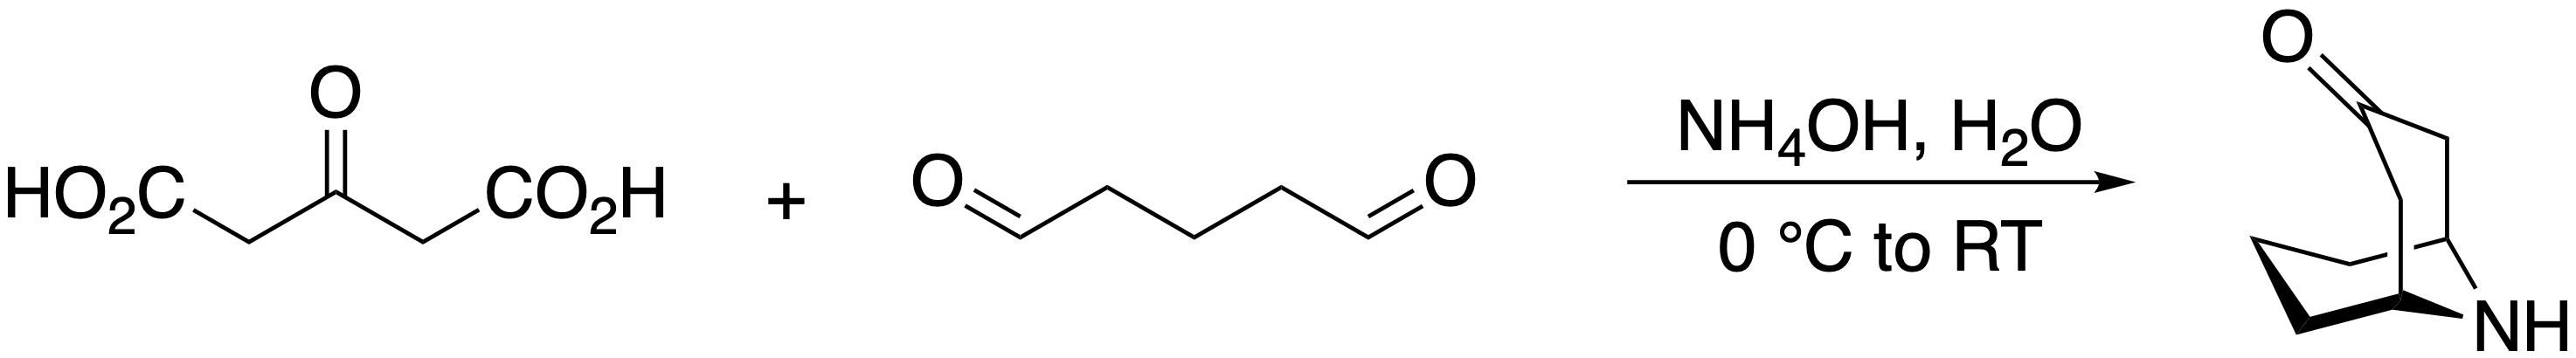
\includegraphics[width=0.6\linewidth]{WPSet1Q1.png}
        \caption{Wendlandt PSet 1, Q1.}
        \label{fig:WPSet1Q1}
    \end{figure}
    \item The reagents: \ce{NH4OH} in water is approximately $\pH=11$.
    \item Keto-enol tautomerization and amine condensation gets the carbons bonded in the right way.
    \begin{itemize}
        \item Dialdehyde forms an imine.
        \item The enol is not unreasonable because hydrogen bonding stabilizes a 6-membered ring.
        \item Then the enol can be a H-bond acceptor from the other carboxylate.
    \end{itemize}
    \item Watch out for reversible steps!!
    \item Loss of \ce{CO2} helps drive some of the steps.
    \item There are multiple right answers; David's sequence of events works, but others could be valid, too.
    \item Aldehyde is more electrophilic than the monoprotonated imine, so if we're gonna react with an imine, we need to change both aldehydes into imines first. Alternatively, we need to diprotonate the imine.
    \item It's not clear whether decarboxylation happens earlier or later in the mechanism.
    \item Altogether, the full solution to PSet 1, Q1 is on the next page.
    \begin{figure}[H]
        \centering
        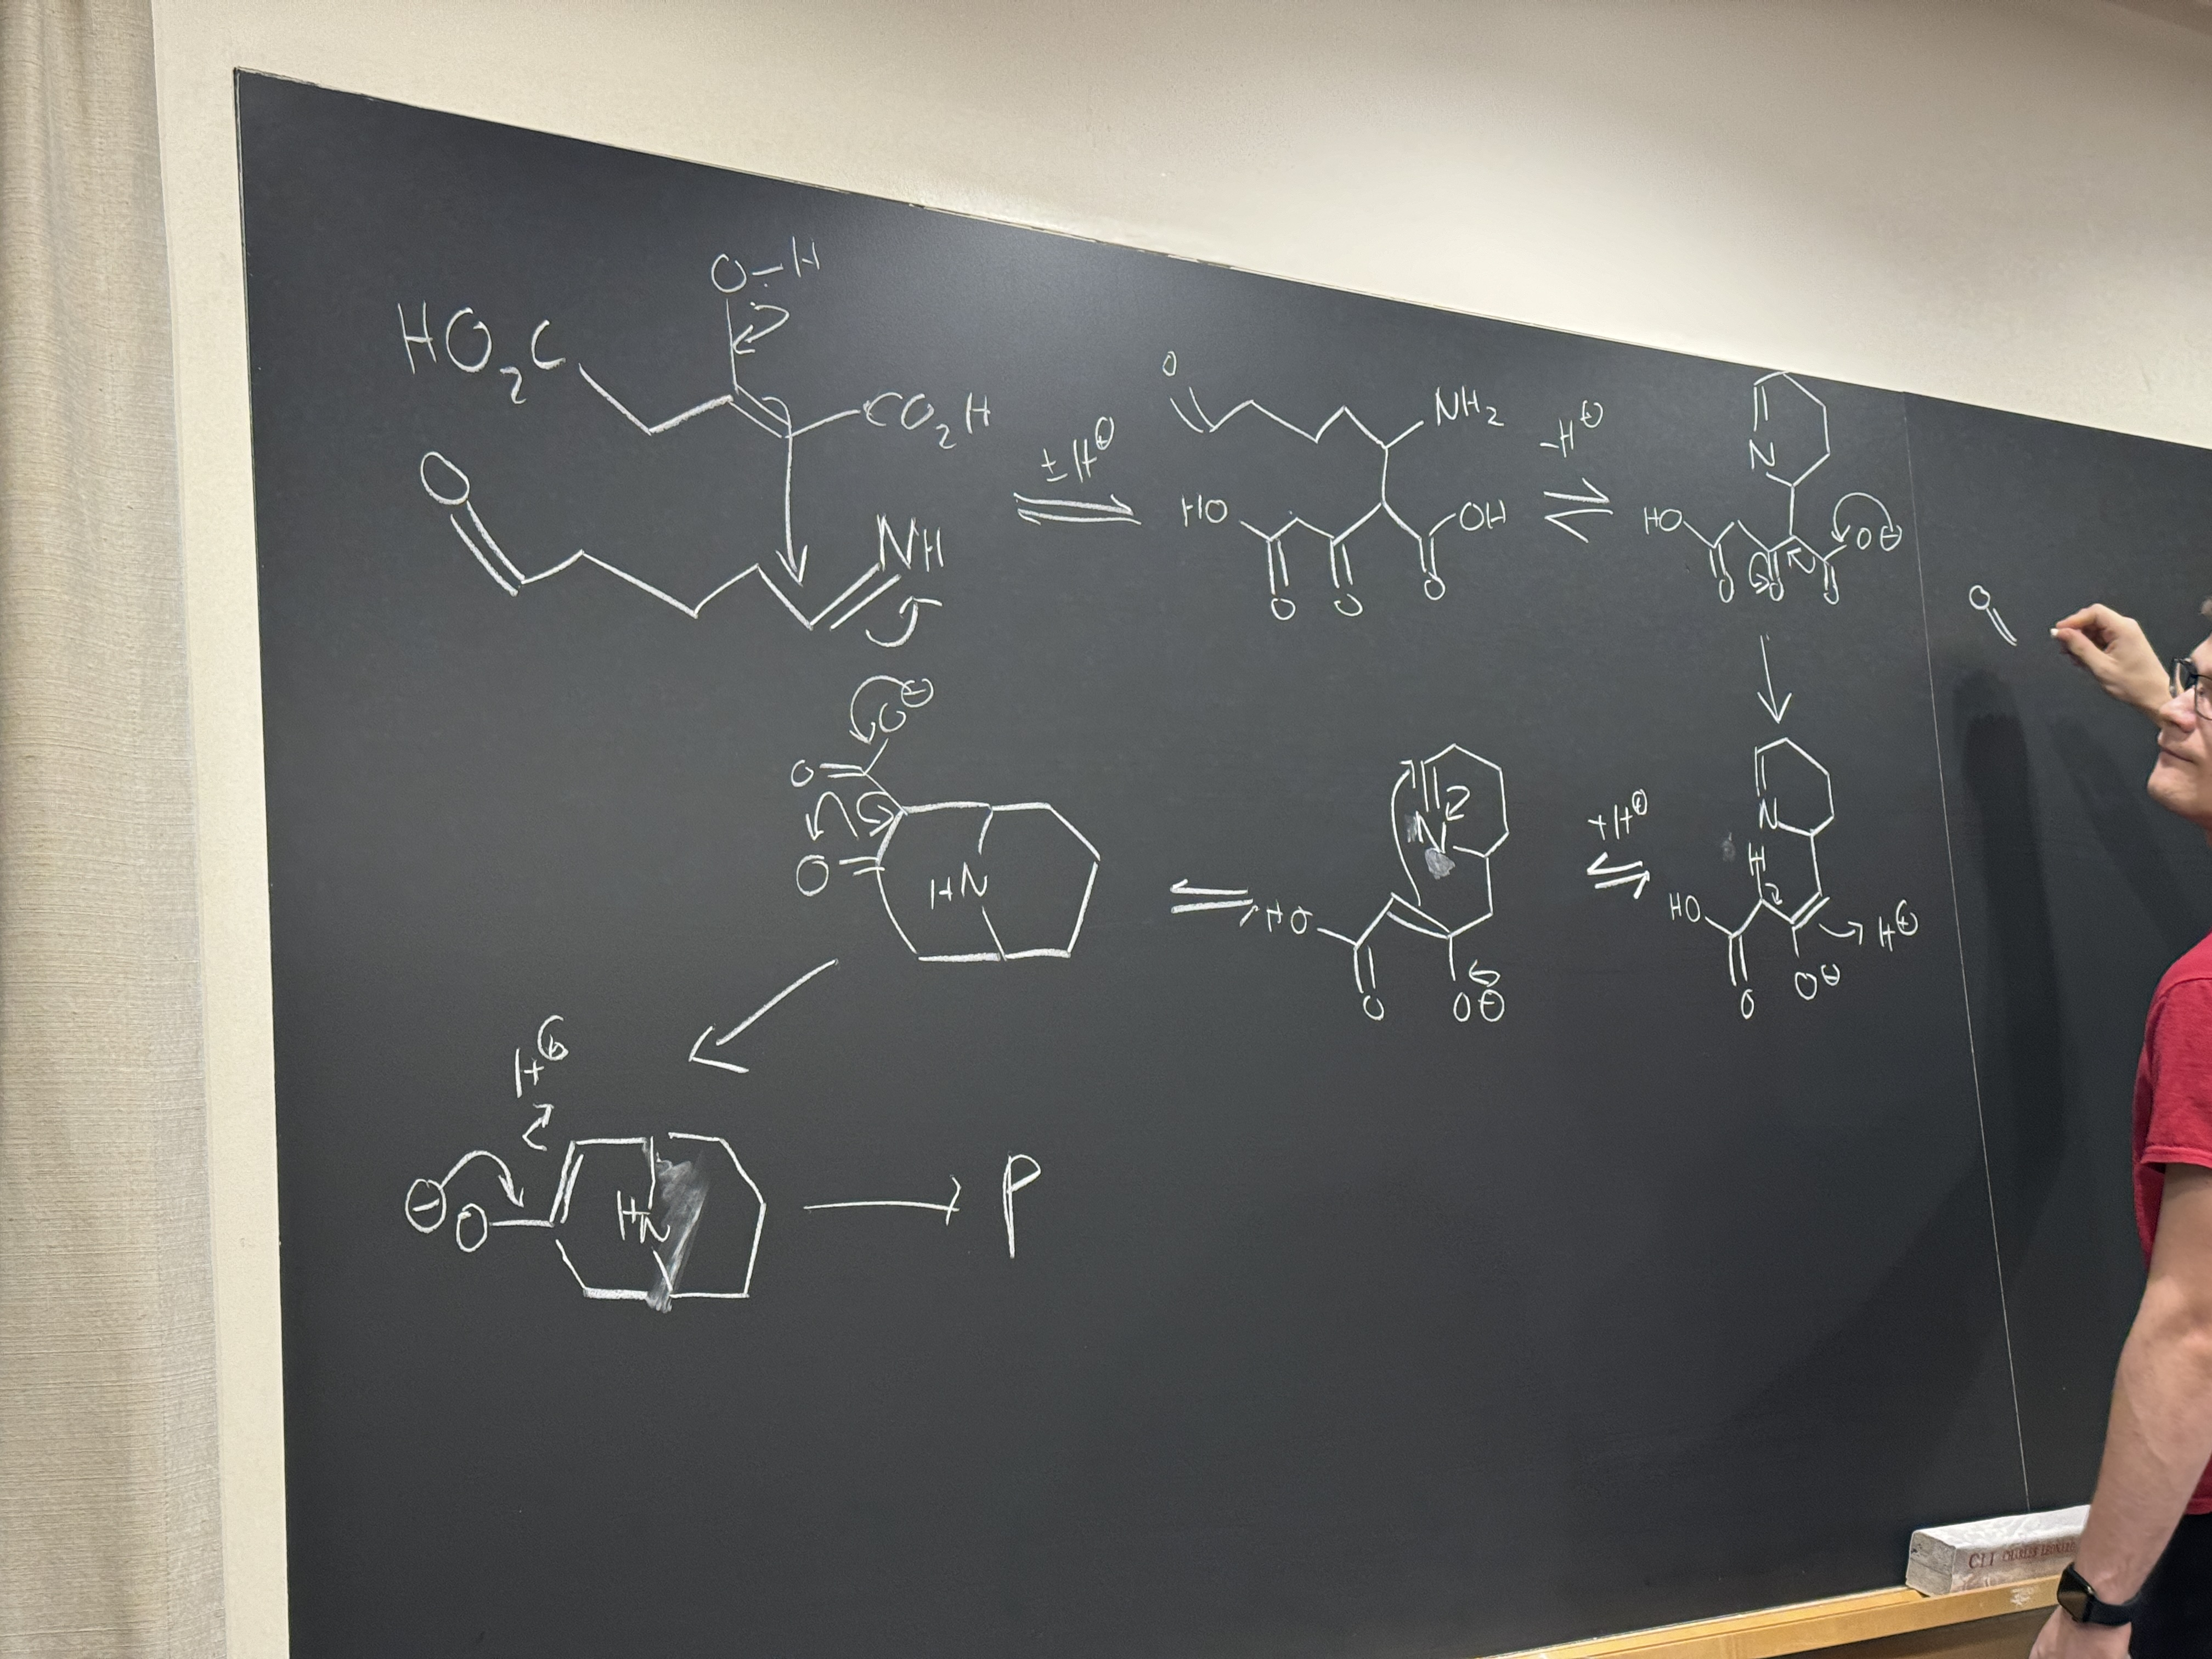
\includegraphics[width=0.8\linewidth]{WPSet1Q1S.JPG}
        \caption{Wendlandt PSet 1, Q1 solution.}
        \label{fig:WPSet1Q1S}
    \end{figure}
    \pagebreak
    \item We now begin discussing Problem 4.
    \begin{figure}[h!]
        \centering
        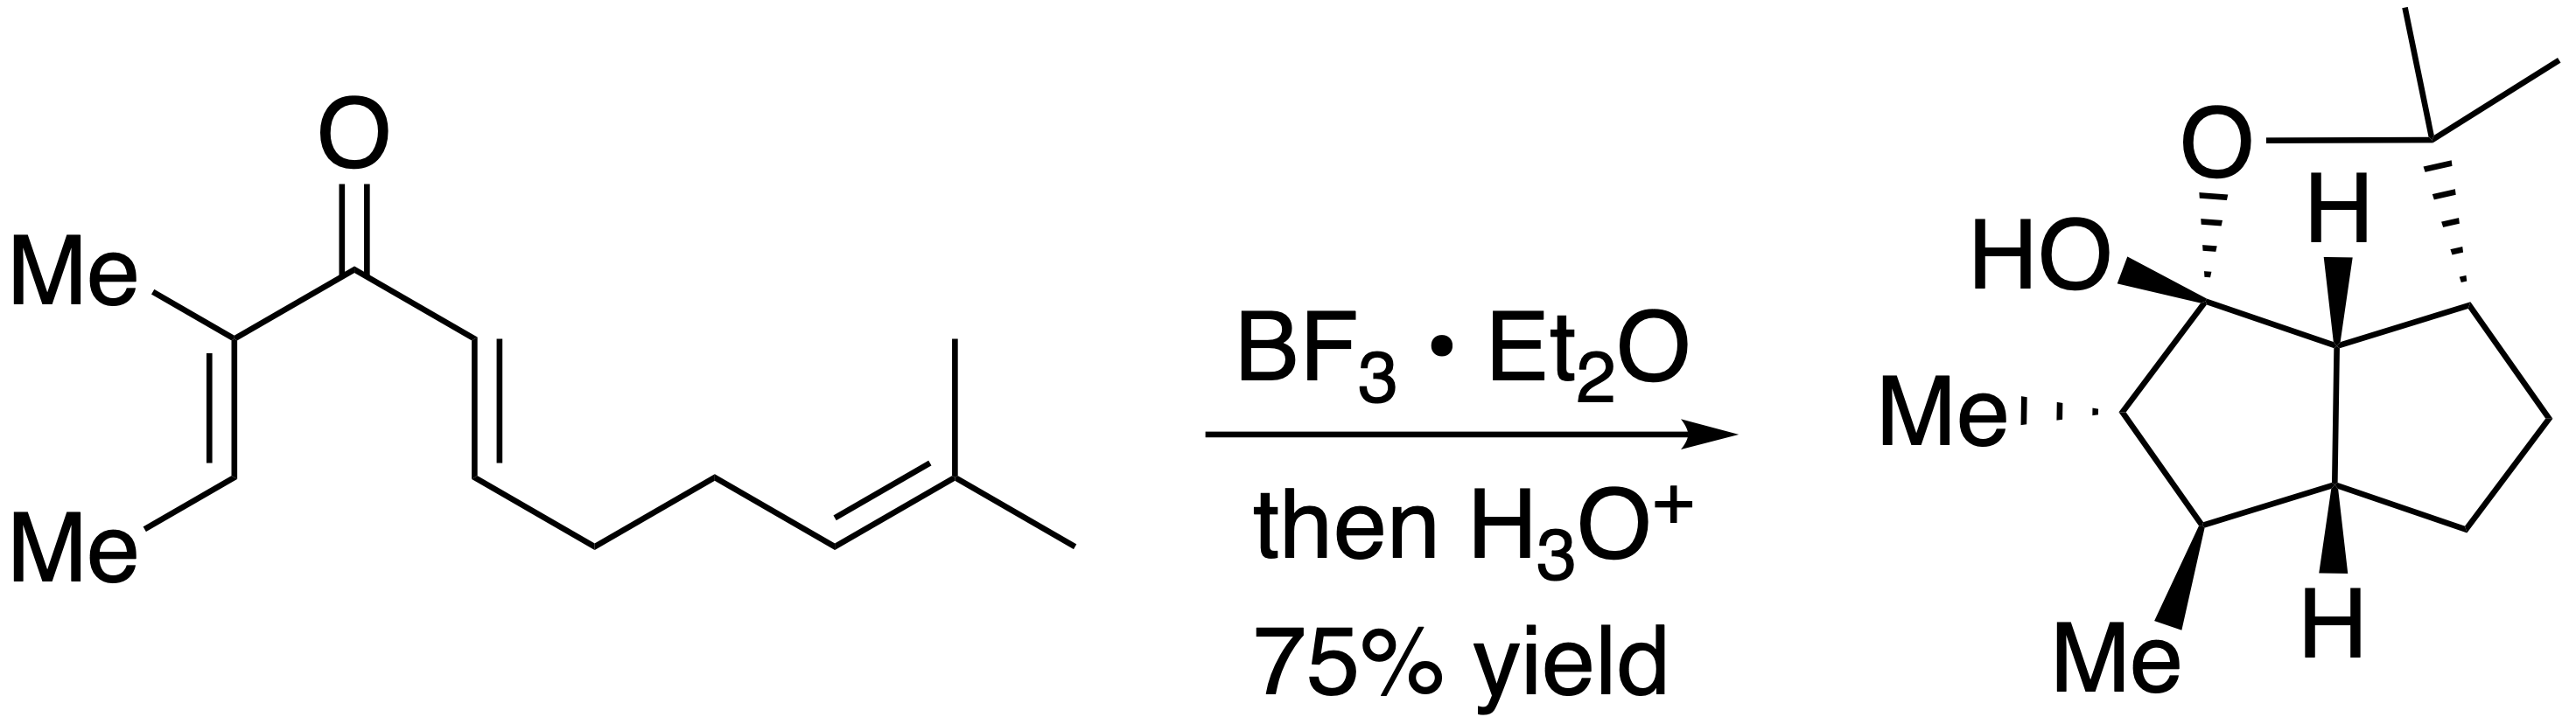
\includegraphics[width=0.45\linewidth]{WPSet1Q4.png}
        \caption{Wendlandt PSet 1, Q4.}
        \label{fig:WPSet1Q4}
    \end{figure}
    \item This is a \textbf{Nazarov reaction}, which is covered in Clayden.
    \item The initial electrocyclization is conrotatory; we need a continuous sequence of $\pi$-orbitals to get this.
    \item The Nazarov is a very powerful tool for making 5-membered rings, but the cation that it leaves oblates a ton of the stereochemical information.
    \item \textbf{Torquoselective reaction}: ...
    \item Orbital analysis yields a structure with the stereochemistry that 
    \item 5,5-trans ring fusions aren't known outside of very unique synthetic constructs. The difference in energy is a huge $\SIrange{5}{7}{\kilo\calorie\per\mole}$.
    \item Scott Denmark has developed strong Lewis acid activation of strong Lewis bases.
    \begin{itemize}
        \item Thus, from the perspective of both the activated Lewis base heteroatom and the perspective of the carbocation, this \ce{C-O} bond-forming reaction should proceed before the acid workup.
    \end{itemize}
    \item Whenever you see a cycloaddition, start thinking about the orbital structure of the HOMO and LUMO.
    \item Altogether, the full solution to PSet 1, Q4 is on the next page.
    \begin{figure}[H]
        \centering
        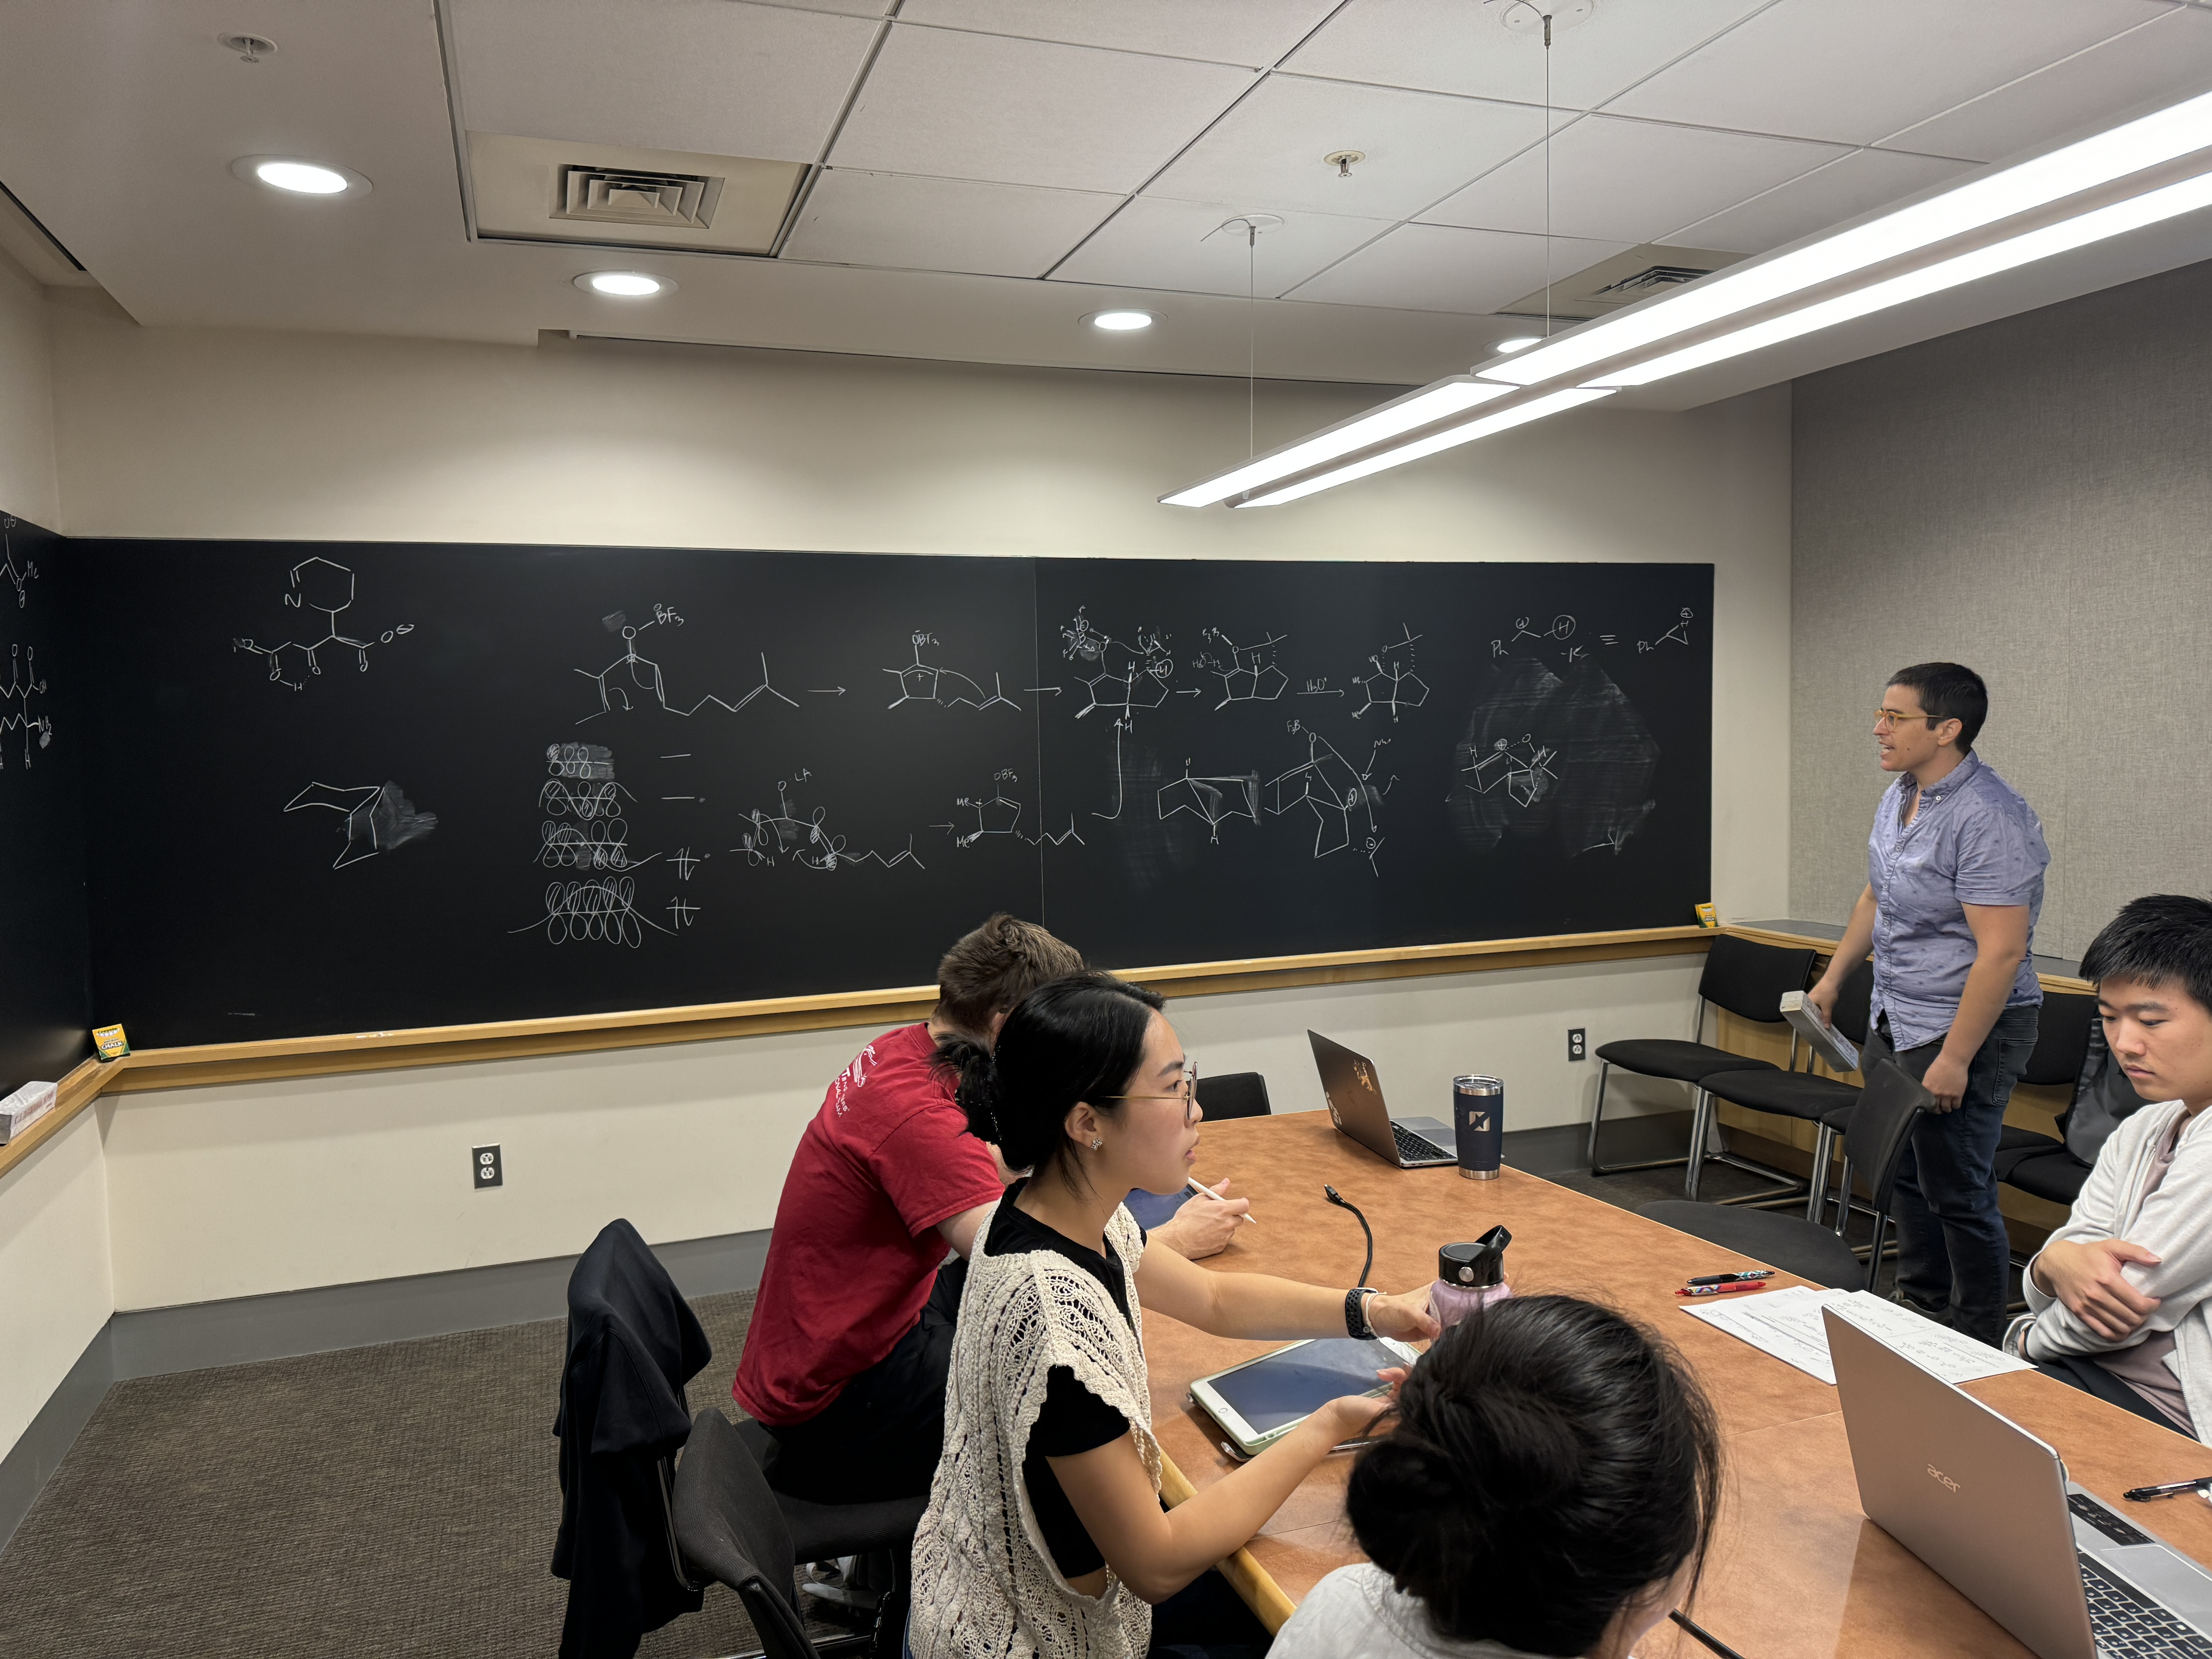
\includegraphics[width=0.8\linewidth]{WPSet1Q4S.JPG}
        \caption{Wendlandt PSet 1, Q4 solution.}
        \label{fig:WPSet1Q4S}
    \end{figure}
    \pagebreak
    \item We now begin discussing Problem 8.
    \begin{figure}[h!]
        \centering
        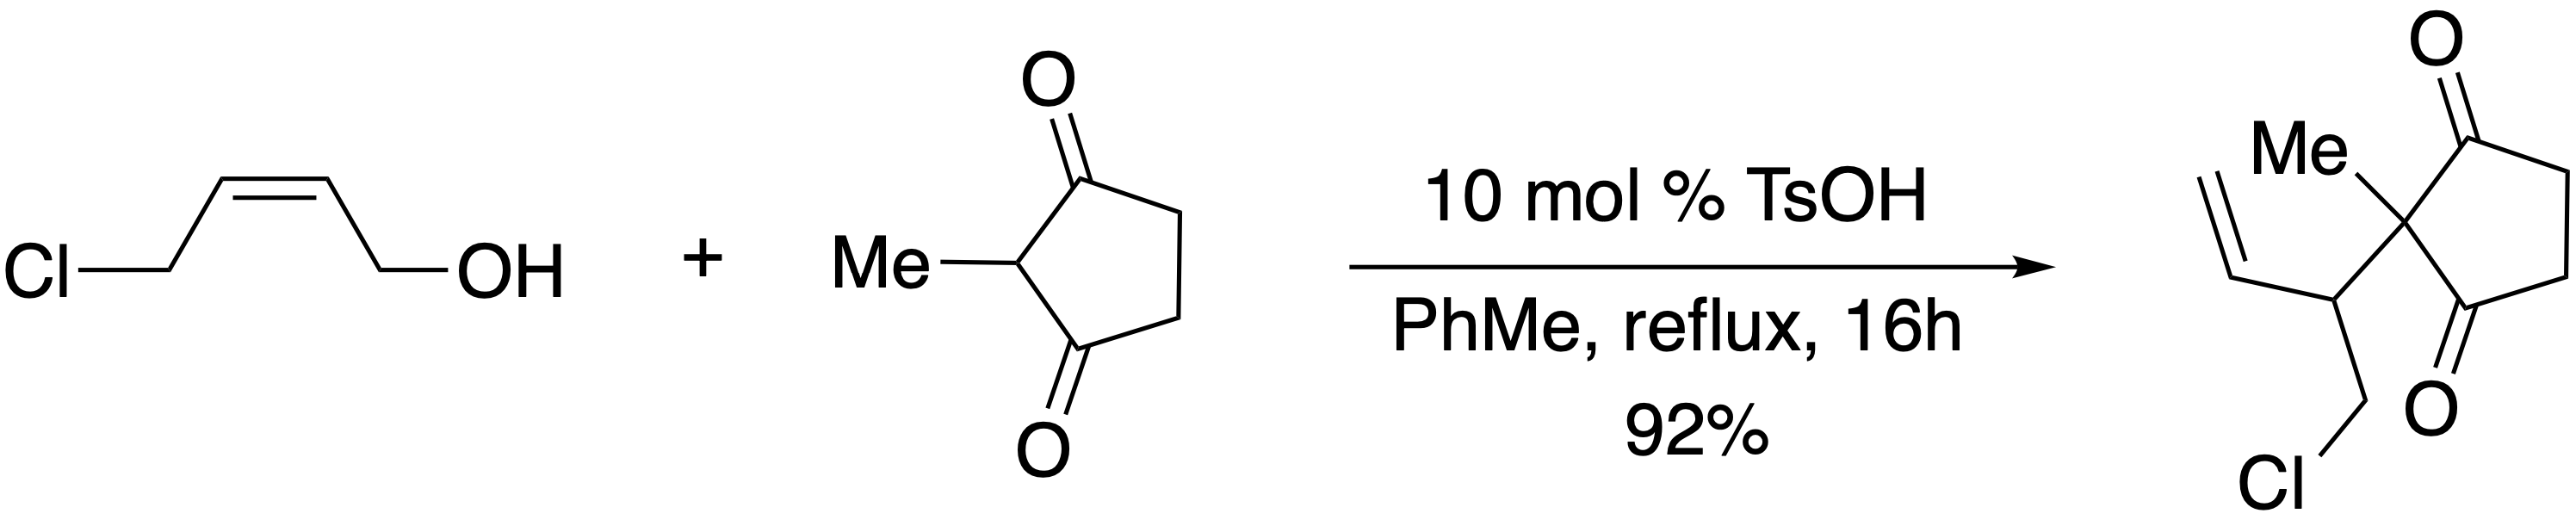
\includegraphics[width=0.6\linewidth]{WPSet1Q8.png}
        \caption{Wendlandt PSet 1, Q8.}
        \label{fig:WPSet1Q8}
    \end{figure}
    \item The thing I proposed is called an S\textsubscript{N}2' reaction, i.e., the attack of one species not on the leaving group but on the conjugated position a couple of carbons away.
    \begin{itemize}
        \item My mechanism is \emph{plausible} but not \emph{defensible}.
        \item The \ce{OH} is not the most Lewis basic species in solution.
    \end{itemize}
    \item Protonating a hemiacetal will be easier than Frank's proposition of protonating the alcohol.
    \begin{itemize}
        \item Alison proposed 1,2-addition and 1,4-addition.
    \end{itemize}
    \item We end with a \textbf{Claisen rearrangement}.
    \item You get a \emph{stabilized} enol structure. Enol is better than enolate for acidic solution.
    \item You use the nucleophilic part to rearrange the electrophilic part.
    \item Altogether, the full solution to PSet 1, Q8 is on the next page.
    \begin{figure}[h!]
        \centering
        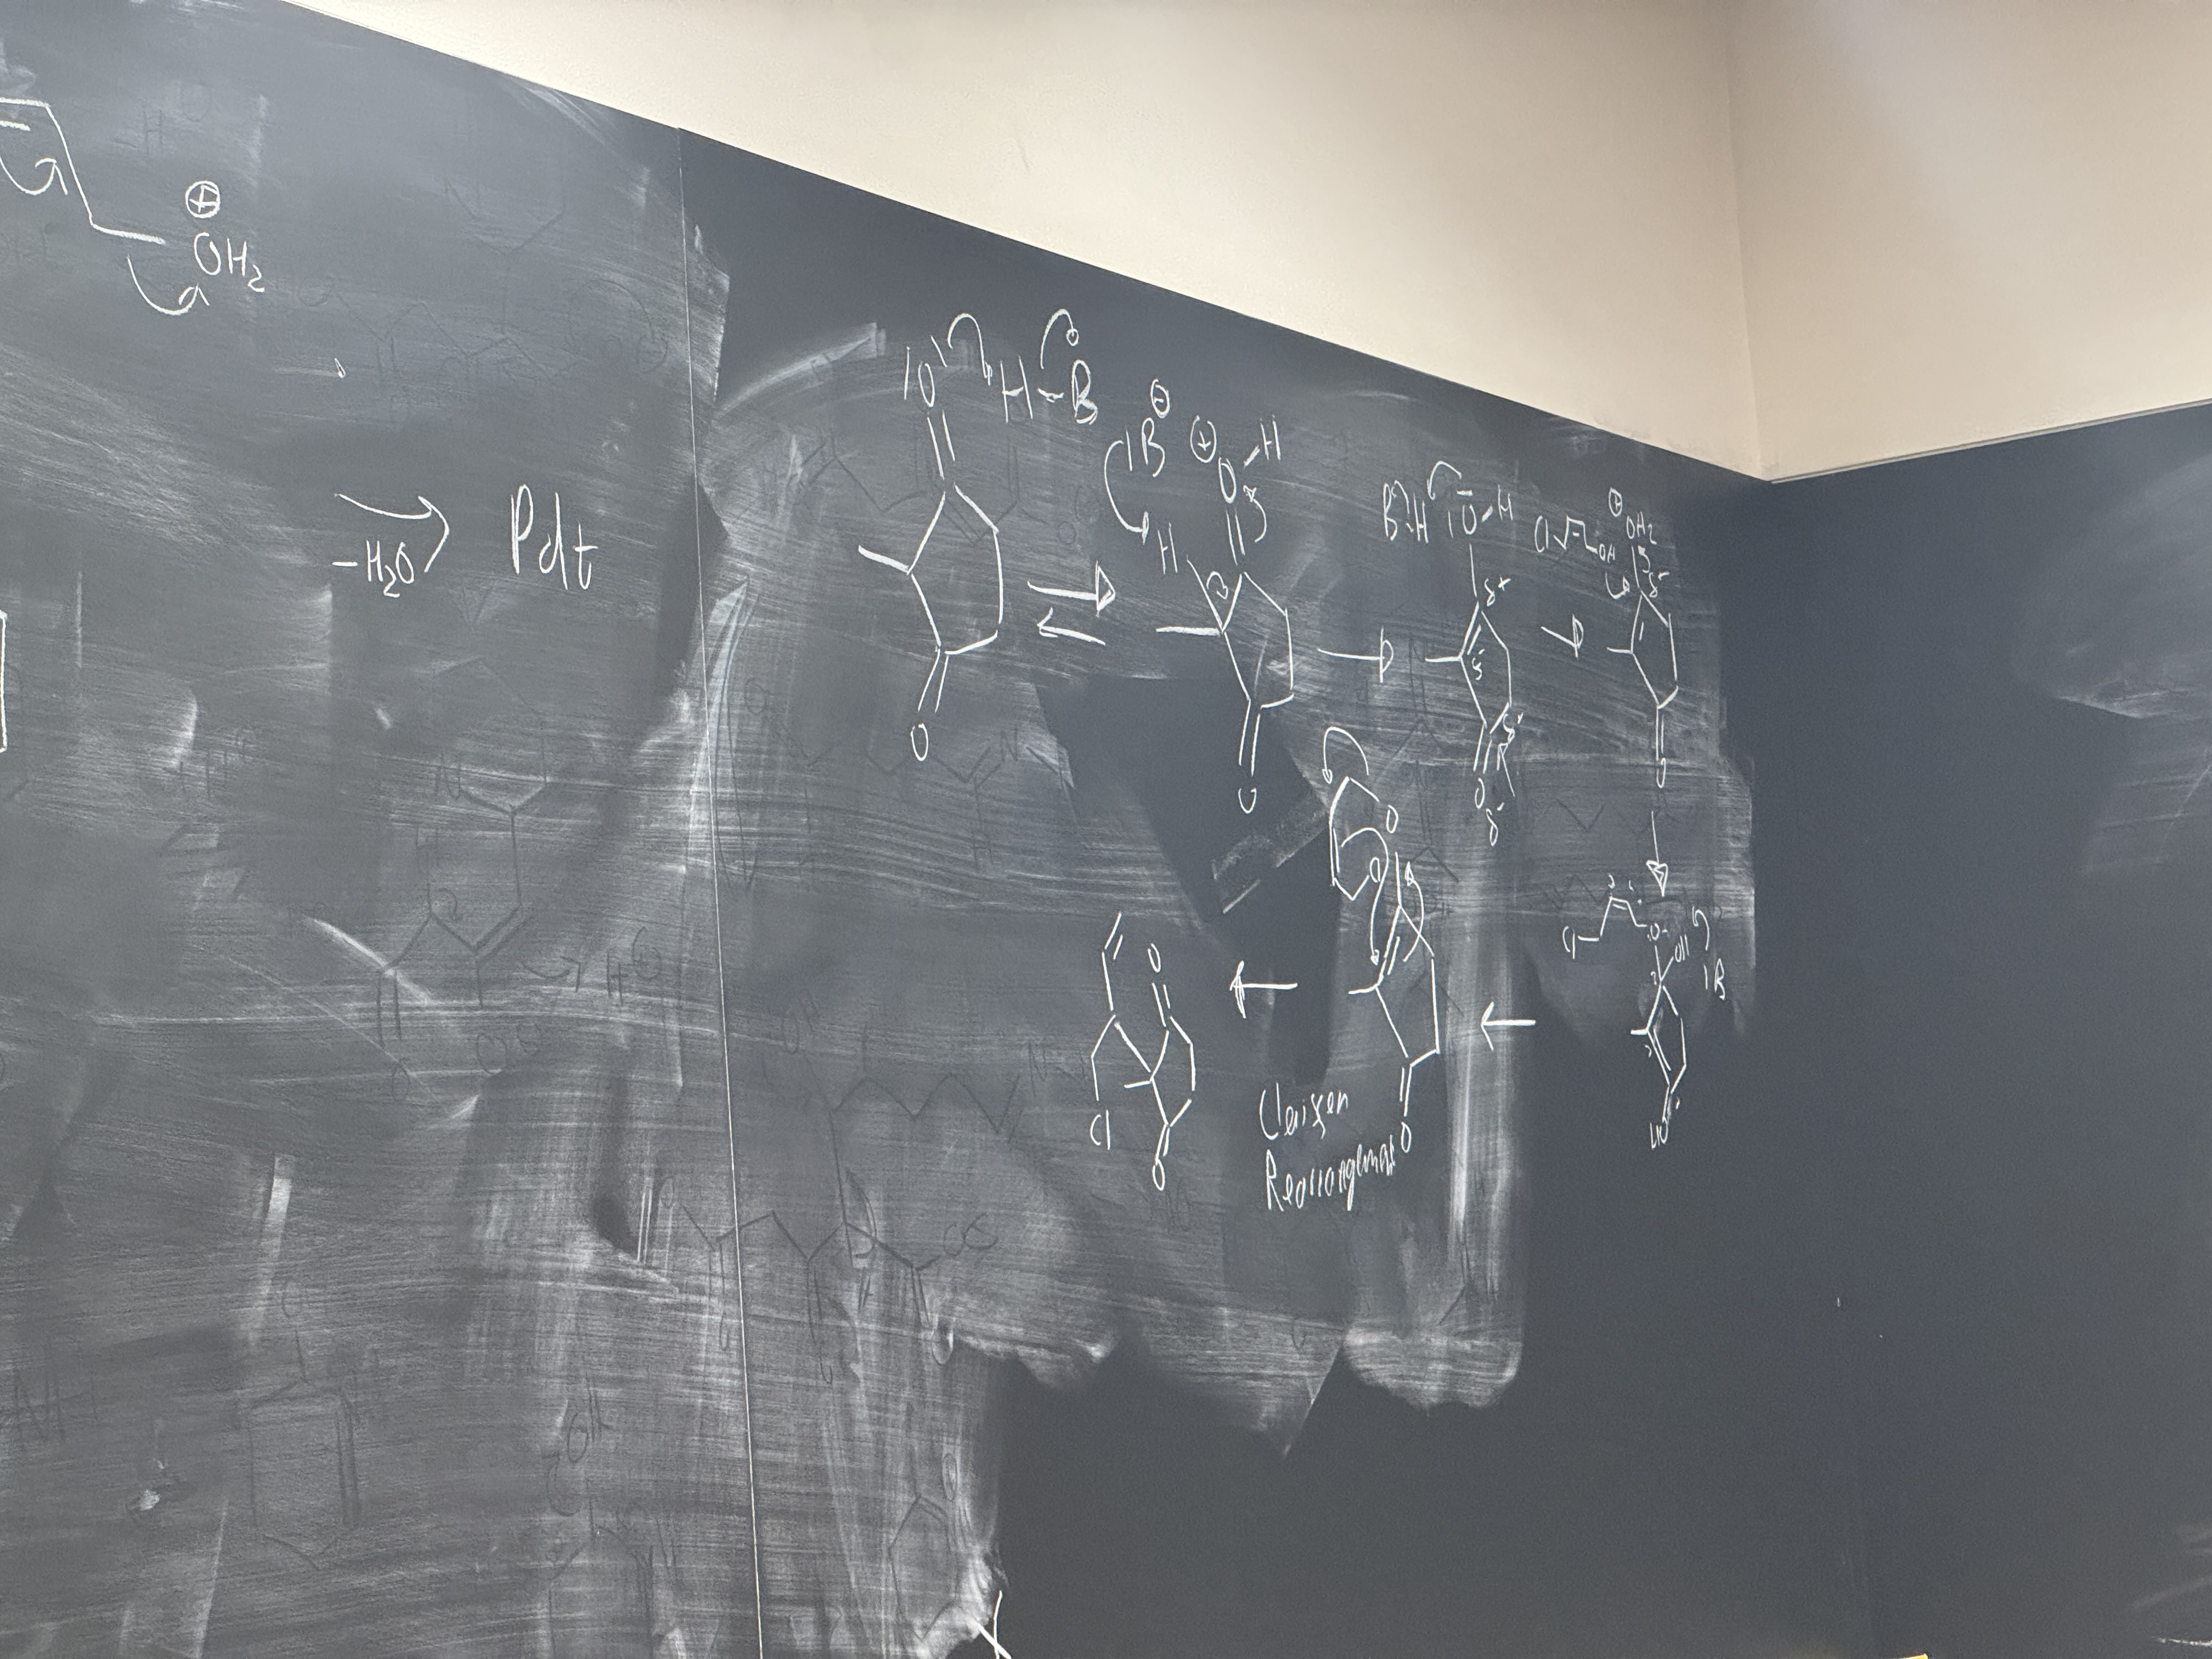
\includegraphics[width=0.8\linewidth]{WPSet1Q8S.JPG}
        \caption{Wendlandt PSet 1, Q8 solution.}
        \label{fig:WPSet1Q8S}
    \end{figure}
\end{itemize}



\section{Problems 3, 5, 6, and 7}
\begin{itemize}
    \item \marginnote{9/18:}Alison used to play ice hockey!
    \item We now begin discussing Problem 6.
    \begin{figure}[h!]
        \centering
        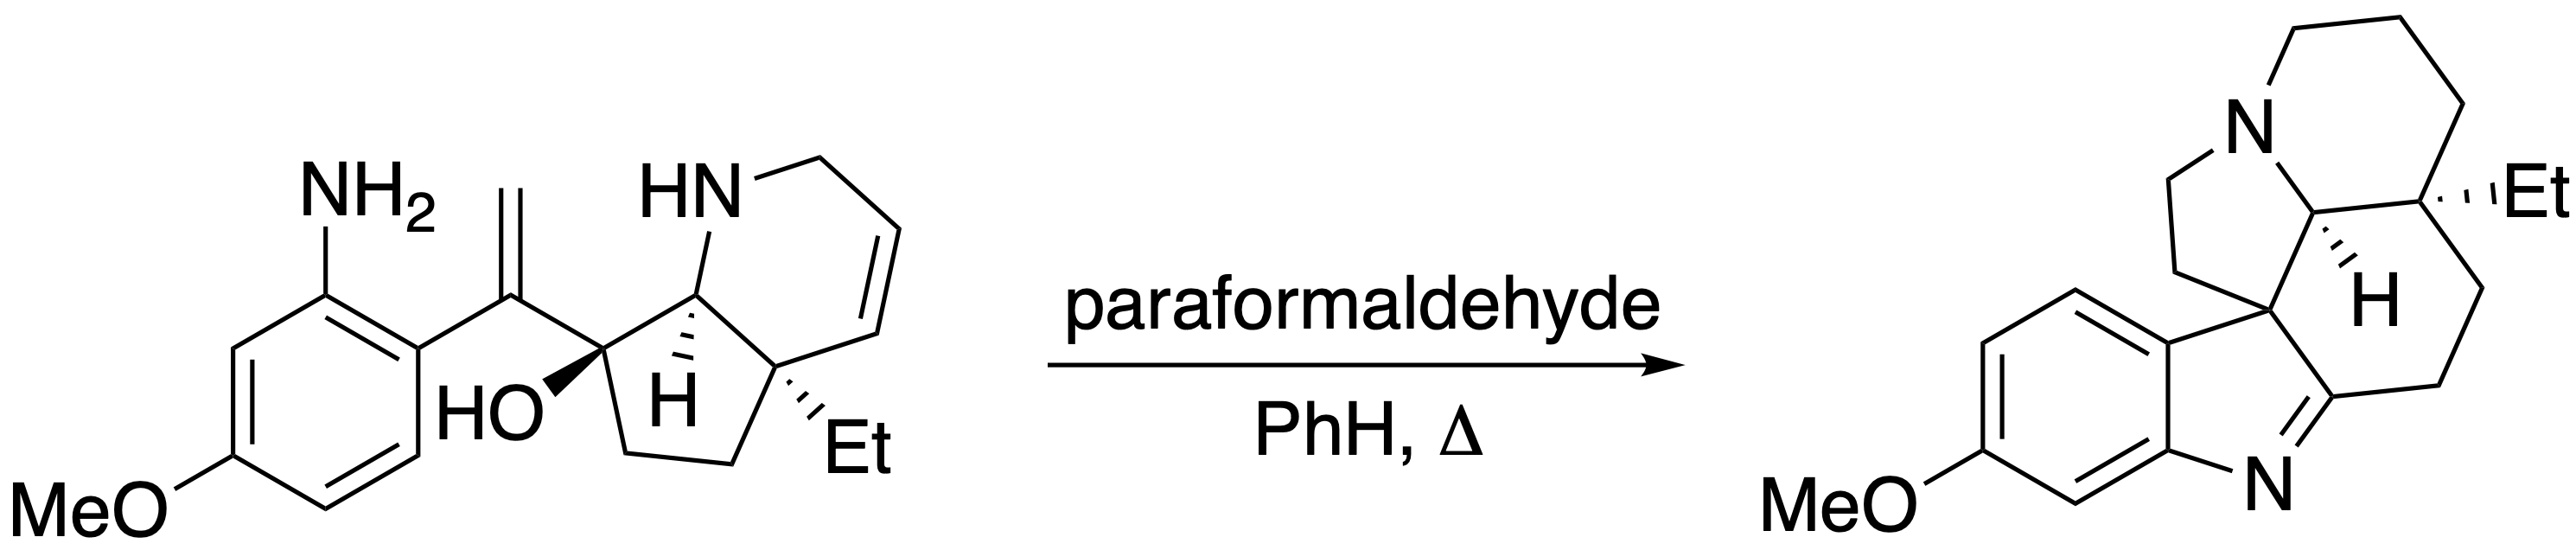
\includegraphics[width=0.6\linewidth]{WPSet1Q6.png}
        \caption{Wendlandt PSet 1, Q6.}
        \label{fig:WPSet1Q6}
    \end{figure}
    \begin{itemize}
        \item I was the only person to have an idea for 6!
        \item There was a typo in the PSet.
    \end{itemize}
    \item \textbf{Sigmatropic step}.
    \begin{itemize}
        \item The $sp^3$ hybrid orbitals become $p$'s. At some point in the transition state, they look $p$-like enough.
        \item It will be \textbf{conrotatory}, so fake substitutents come out on the same side.
        \item Don't remember the rules; just draw the orbitals and figure it out.
        \item David's pneumonic: 64 disco: 6 disrotatory, 4 conrotatory. Then for light, you just reverse it.
    \end{itemize}
    \item Does everything happen very quickly, or do things pull apart first and we tautomerize to a ketone before we go back to an enol and react.
    \item Nonpolar solvent and high temperature often implies pericyclic reaction!
    \item Where are acids and bases coming from? The molecule itself? How does the condensation occur?
    \begin{itemize}
        \item Protonated piperidine: $\pKa=10$.
        \item Protonated aniline: $\pKa=8$.
        \item Learn the \href{http://ccc.chem.pitt.edu/wipf/MechOMs/evans_pKa_table.pdf}{Evans} $\pKa$ table!!
        \item The aniline probably forms the iminium with the formaldehyde, and that's just reversible until we can do the entropically favorable step.
    \end{itemize}
    \item Altogether, the full solution to PSet 1, Q6 is on the next page.
    \begin{figure}[H]
        \centering
        \begin{subfigure}[b]{\linewidth}
            \centering
            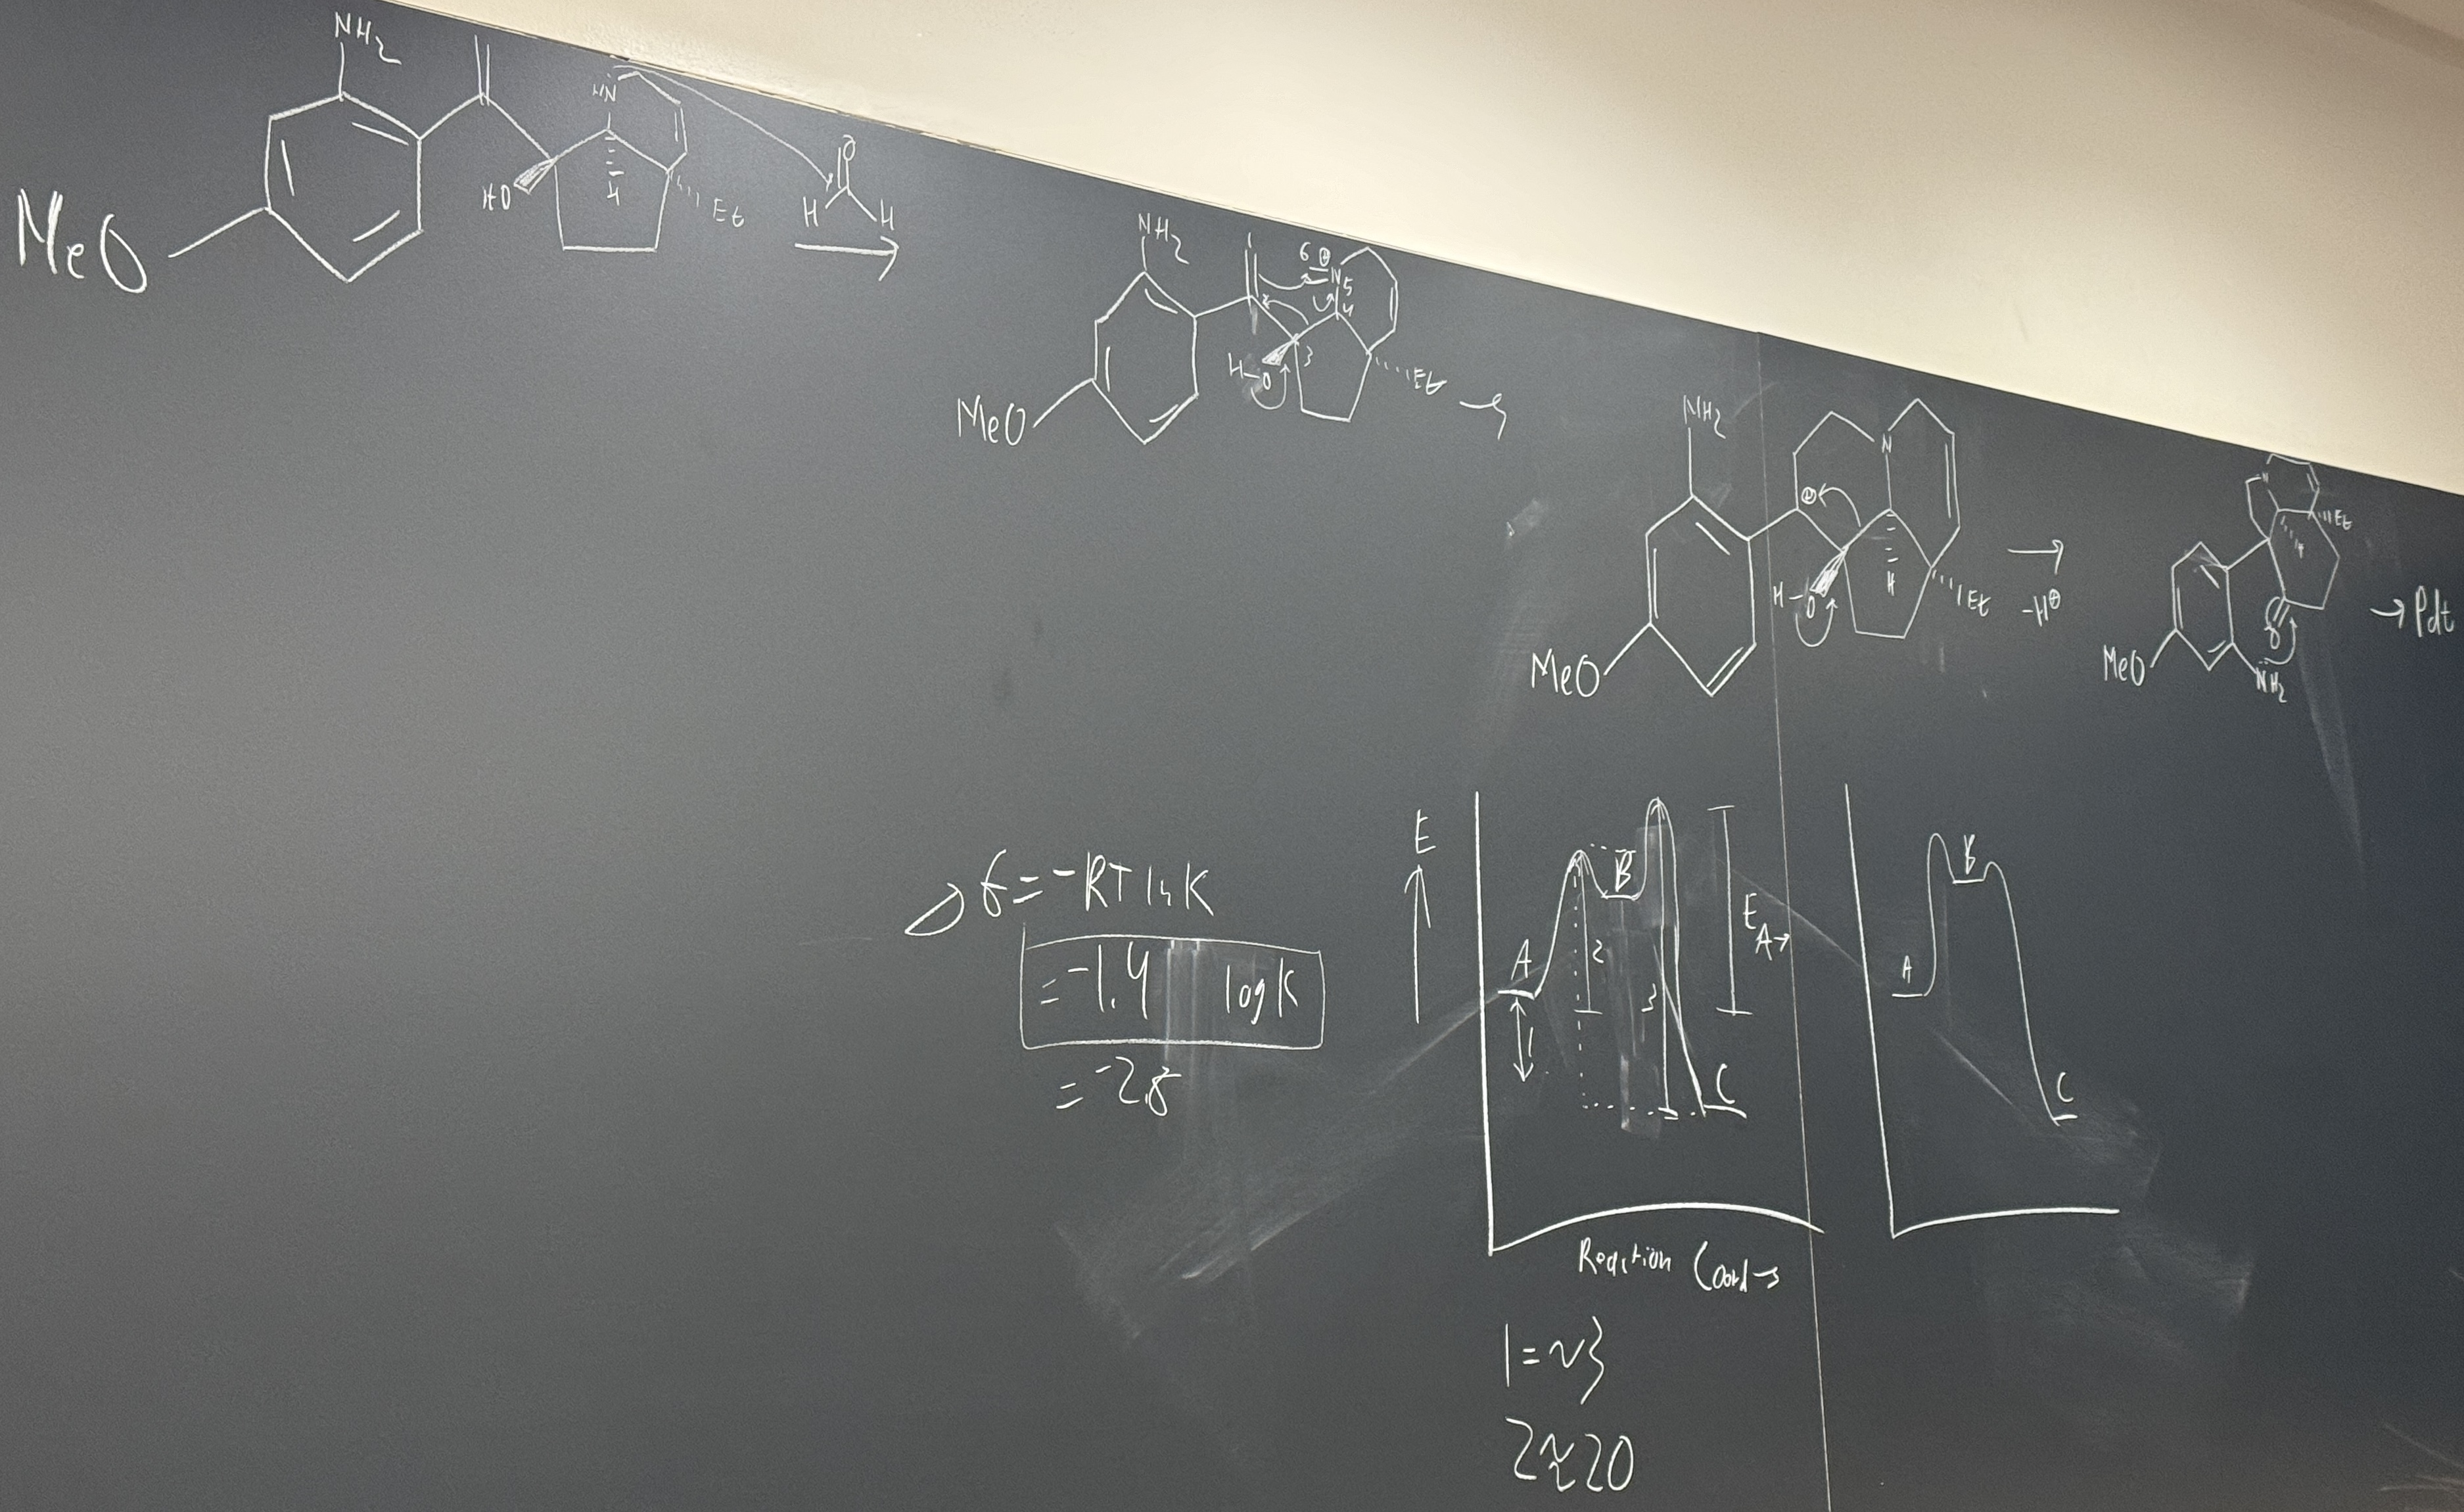
\includegraphics[width=0.8\linewidth]{WPSet1Q6Sa.JPG}
            \caption{My proposition.}
            \label{fig:WPSet1Q6Sa}
        \end{subfigure}\\[2em]
        \begin{subfigure}[b]{\linewidth}
            \centering
            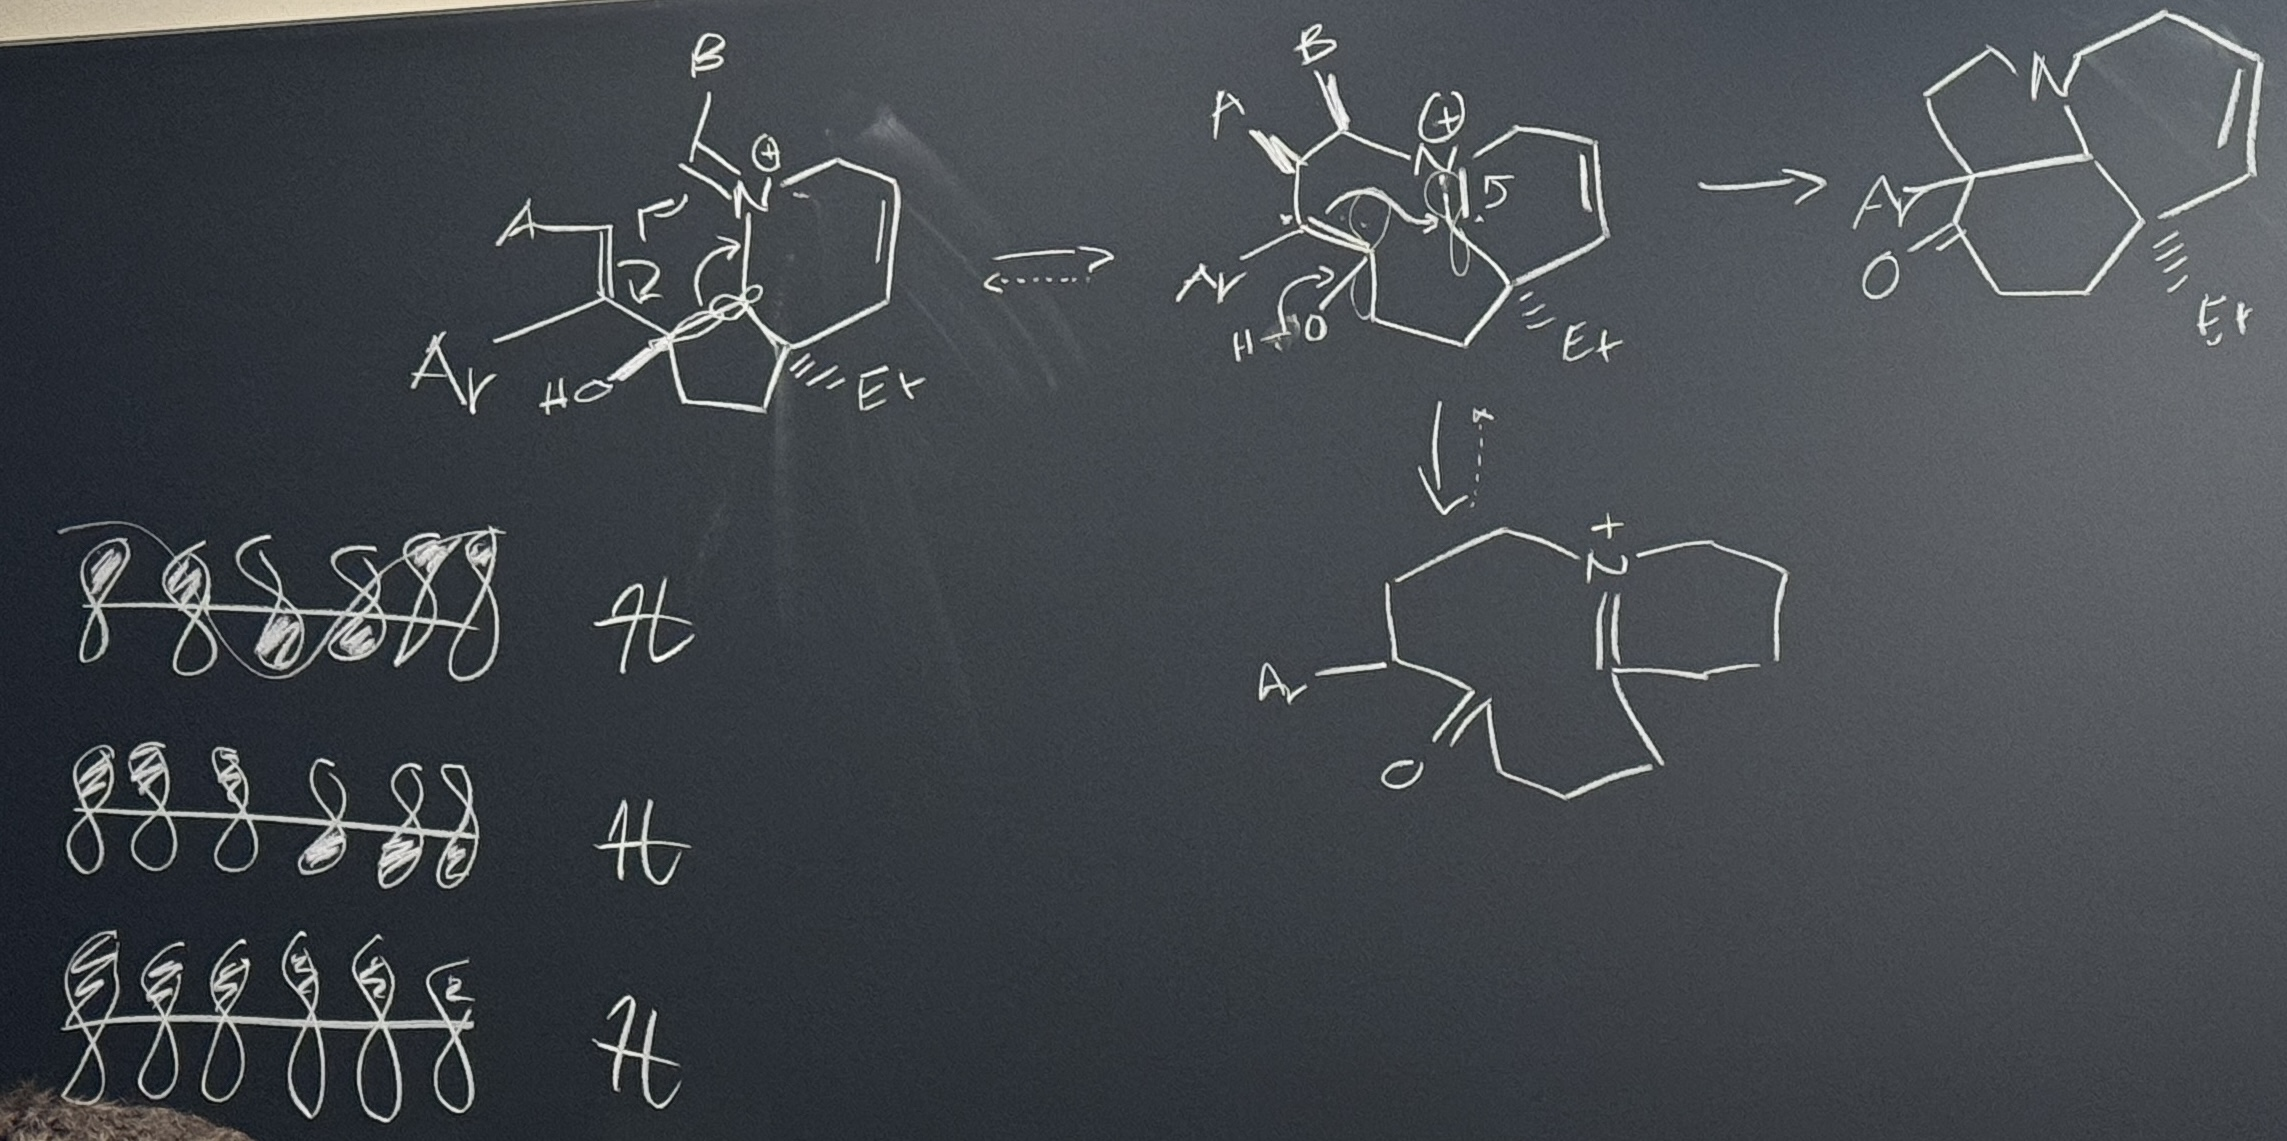
\includegraphics[width=0.8\linewidth]{WPSet1Q6Sb.JPG}
            \caption{Sigmatropic correction.}
            \label{fig:WPSet1Q6Sb}
        \end{subfigure}
        \caption{Wendlandt PSet 1, Q6 solution.}
        \label{fig:WPSet1Q6S}
    \end{figure}
    \pagebreak
    \item We now begin discussing Problem 7.
    \begin{figure}[h!]
        \centering
        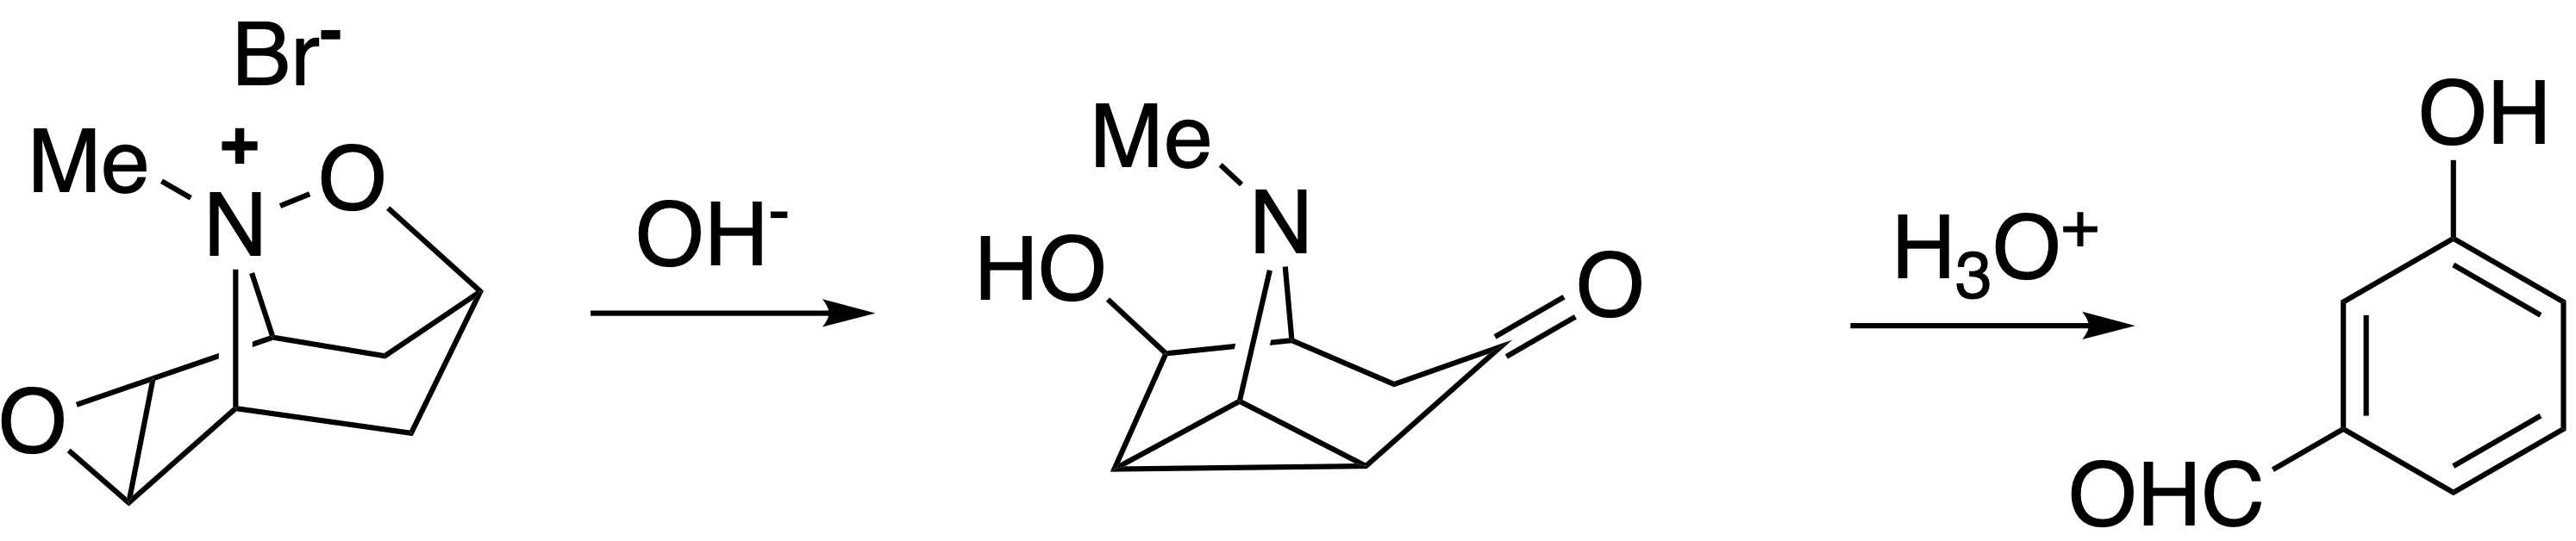
\includegraphics[width=0.5\linewidth]{WPSet1Q7.png}
        \caption{Wendlandt PSet 1, Q7.}
        \label{fig:WPSet1Q7}
    \end{figure}
    \item Somebody prepared a beautiful molecule, and then it just decomposed into this basic AF benzaldehyde derivative.
    \item This is probably a classic case of working in a lab, finding the decomposition product, going back to your PI, and then having to resort to arrow pushing to figure out what happened.
    \item The first step is helped by an antiperiplanar arrangement and the fact that the iminium wants its electron pair back.
    \item Altogether, the full solution to PSet 1, 7 is on the next page.
    \begin{figure}[h!]
        \centering
        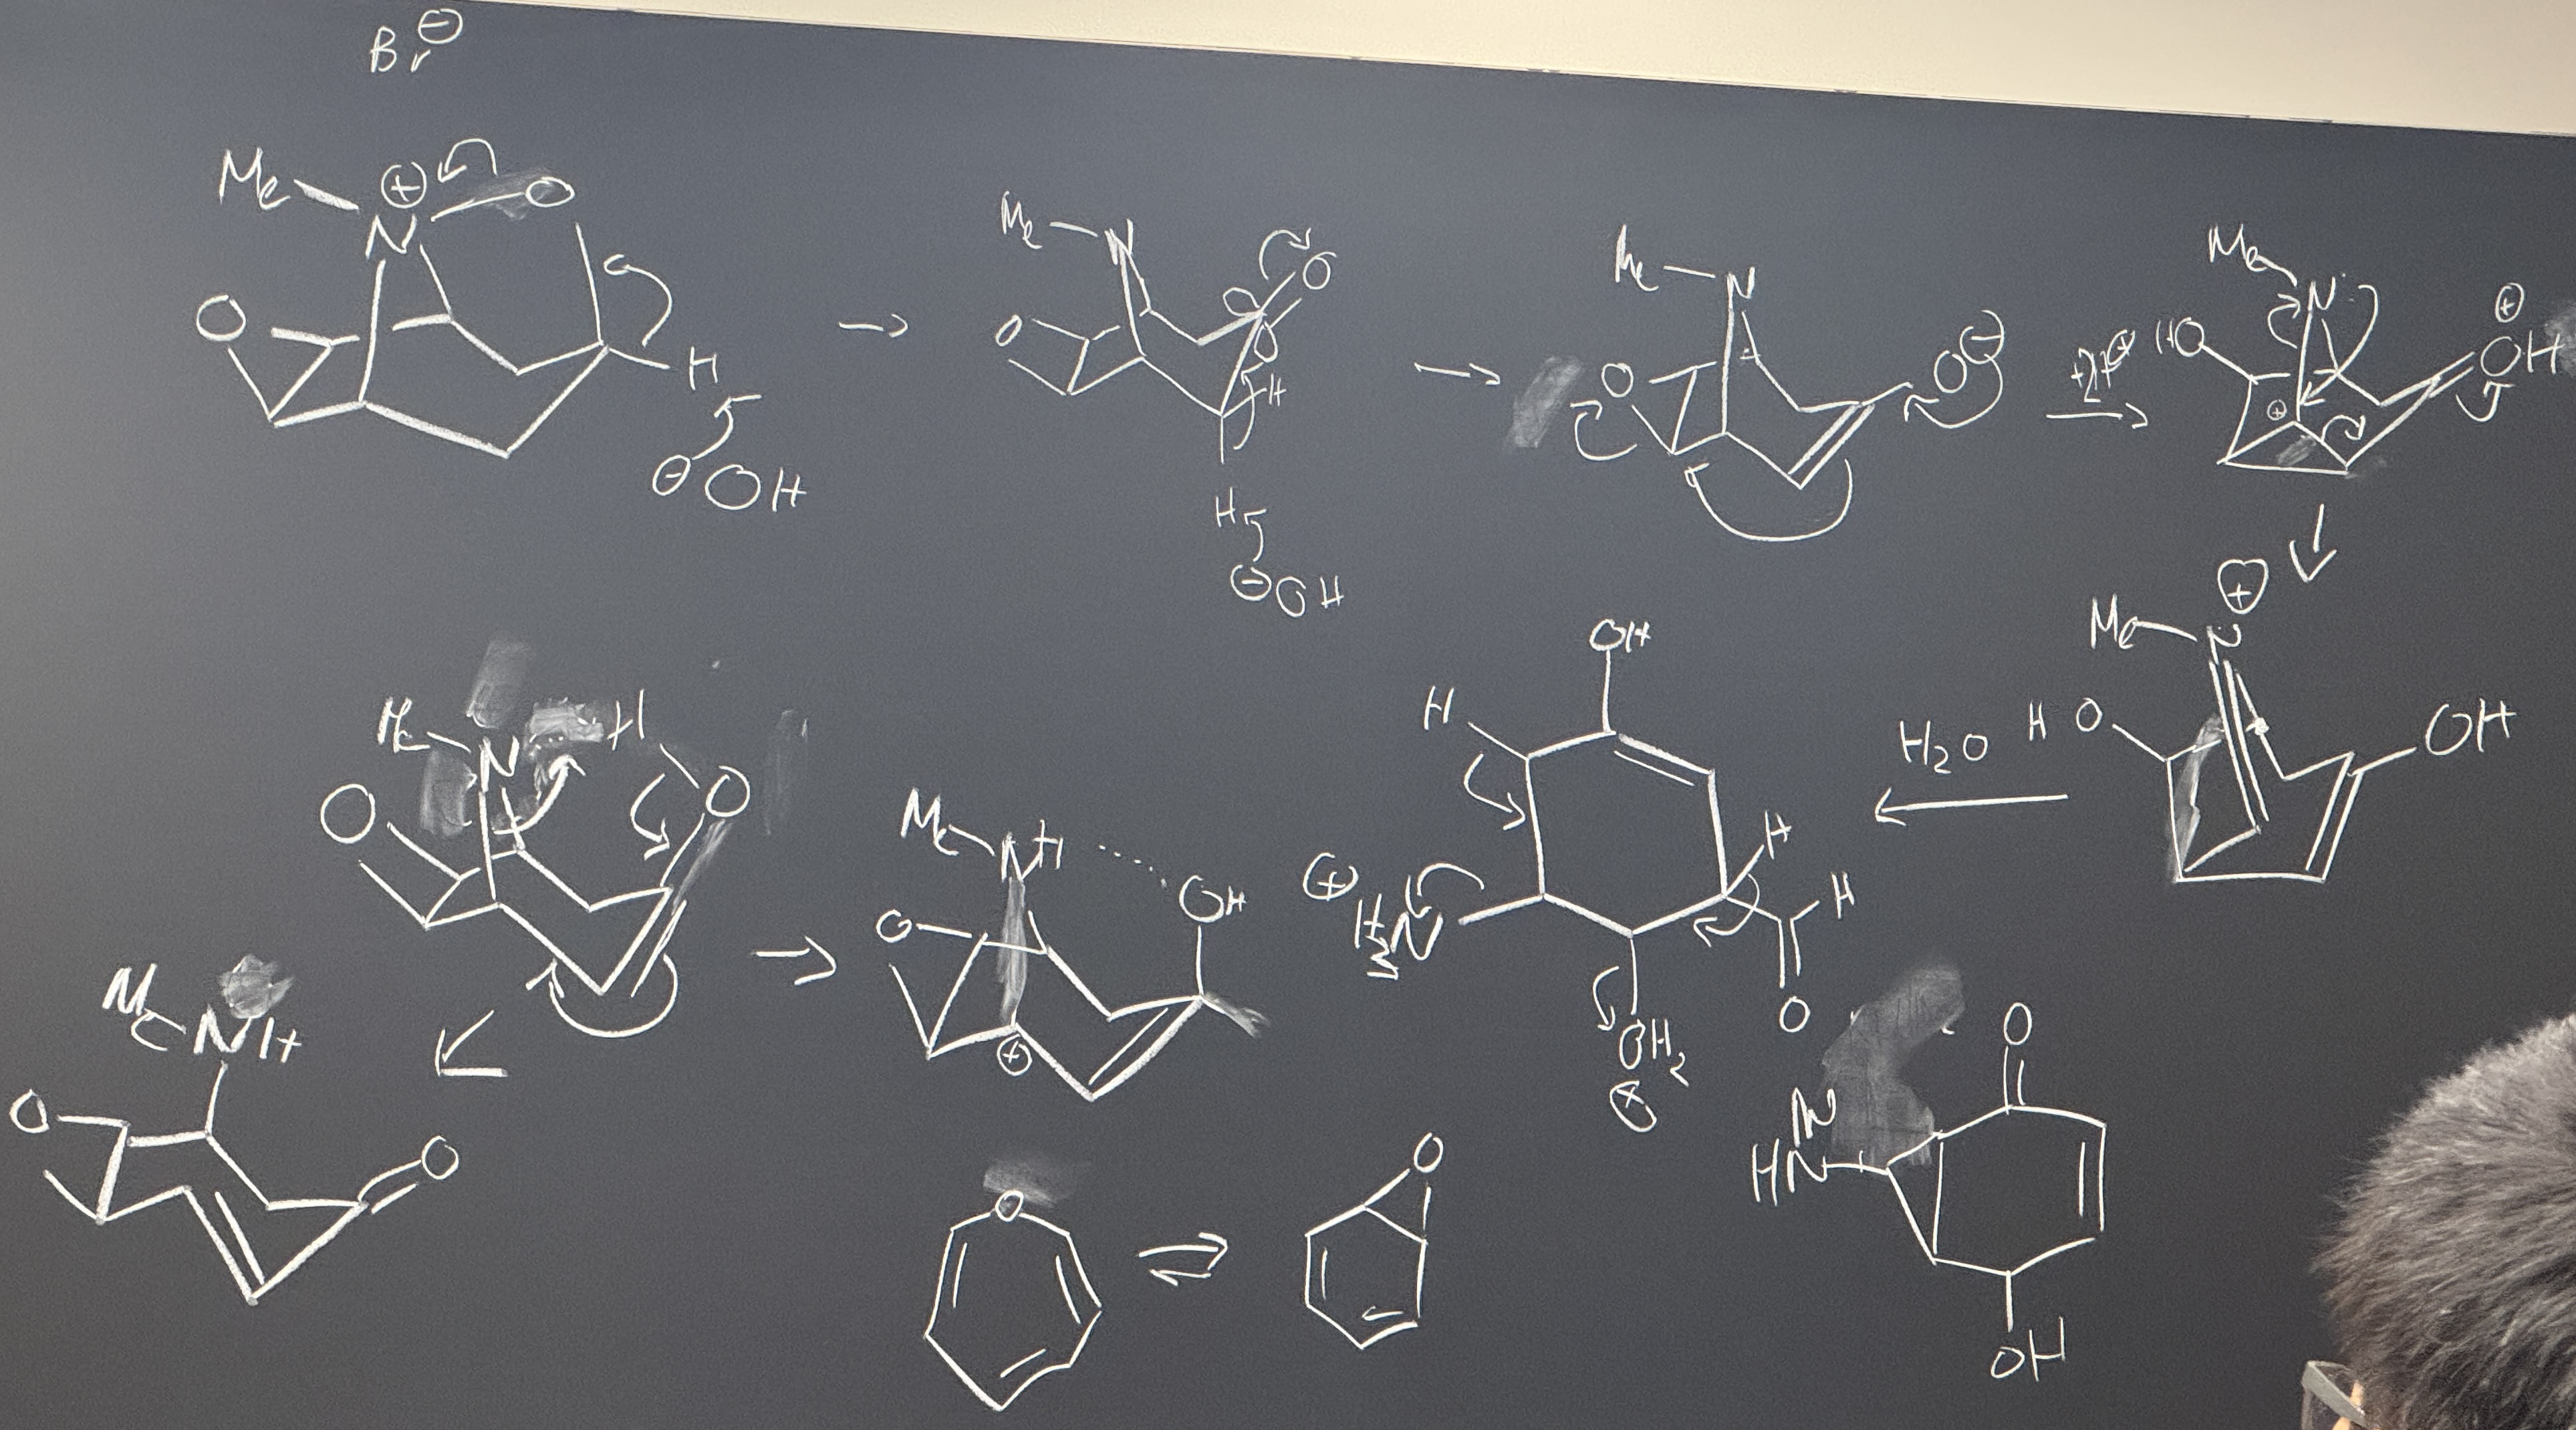
\includegraphics[width=0.8\linewidth]{WPSet1Q7S.JPG}
        \caption{Wendlandt PSet 1, Q7 solution.}
        \label{fig:WPSet1Q7S}
    \end{figure}
    \pagebreak
    \item We now begin discussing Problem 5.
    \begin{figure}[h!]
        \centering
        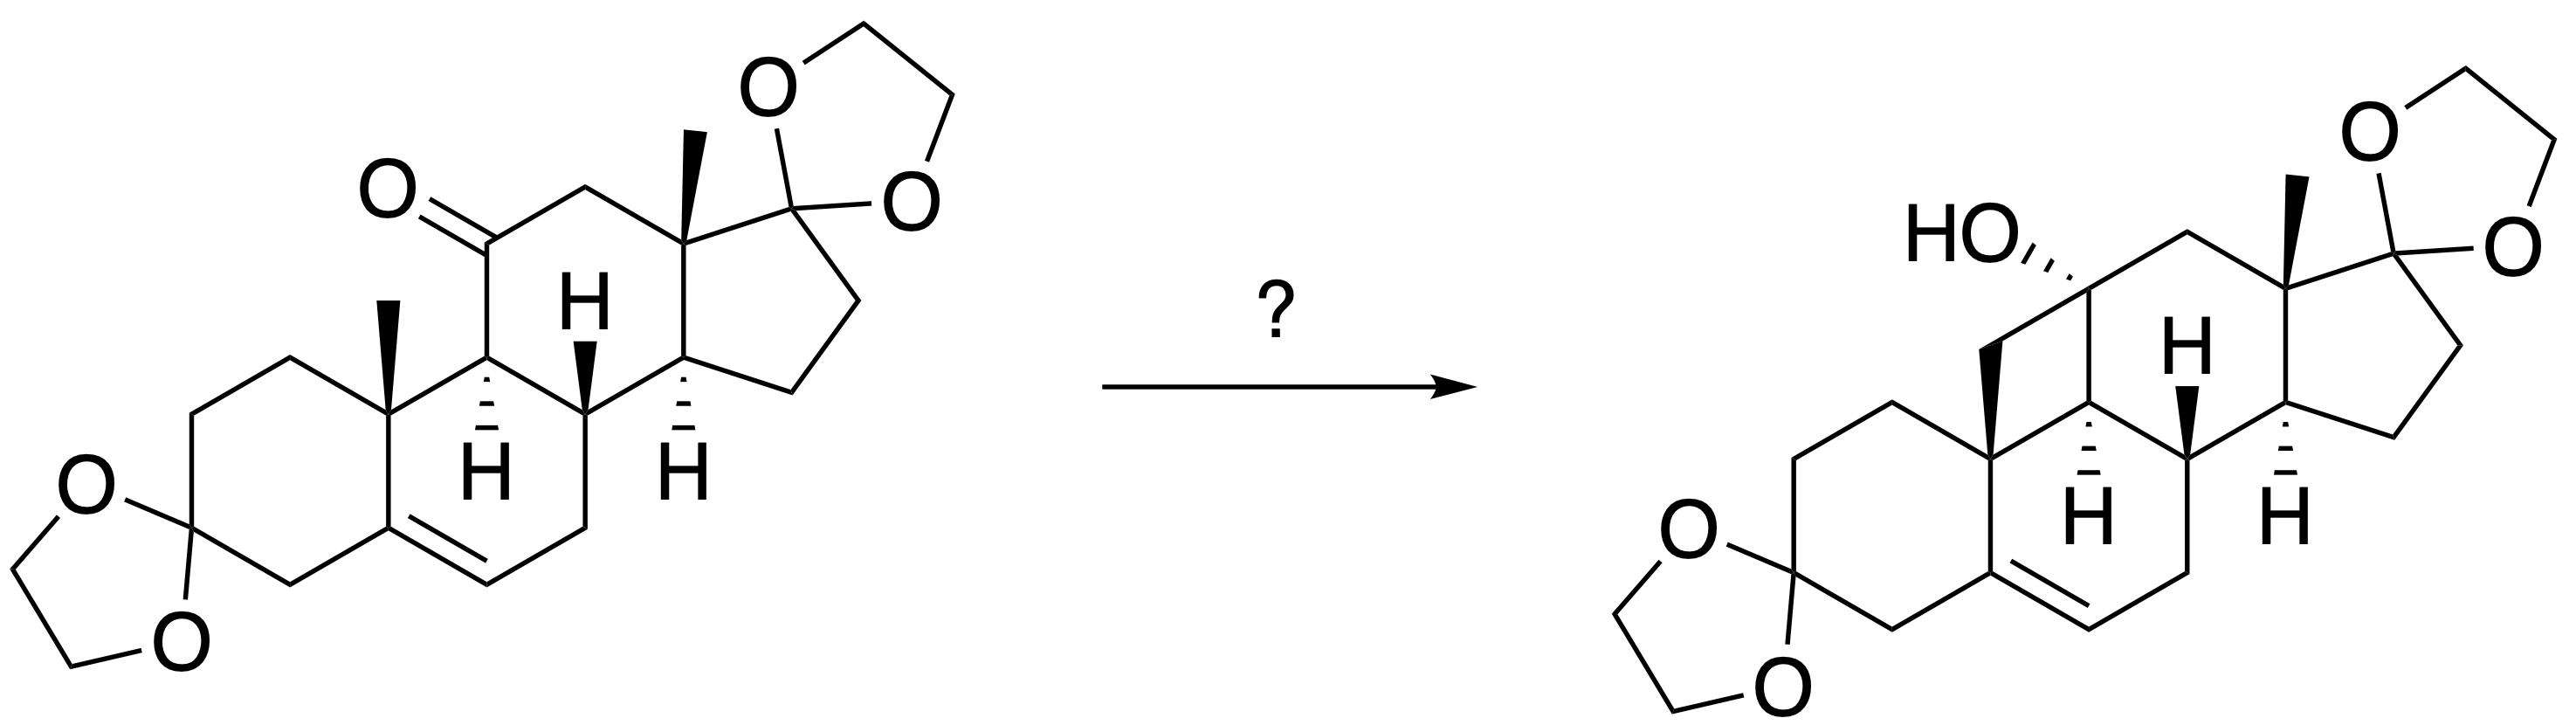
\includegraphics[width=0.55\linewidth]{WPSet1Q5.png}
        \caption{Wendlandt PSet 1, Q5.}
        \label{fig:WPSet1Q5}
    \end{figure}
    \item \textbf{Noorish 2 reaction}.
    \item Why is \ce{O*} less stable than \ce{C*}?
    \begin{itemize}
        \item Bond dissociation energies.
        \item \SI{10}{\kilo\calorie\per\mole} driving force to form \ce{O-H} and break \ce{C-H}.
        \item \SI{50}{\kilo\calorie\per\mole} favorability for deprotonating isopropanol at the alcohol vs. the methine \ce{C-H}.
        \begin{itemize}
            \item Derived by 35-fold difference in $\pKa$, so $\Delta G=-1.4\log(10^{35})\approx 50$.
        \end{itemize}
    \end{itemize}
    \item Altogether, the full solution to PSet 1, Q5 is on the next page.
    \begin{figure}[h!]
        \centering
        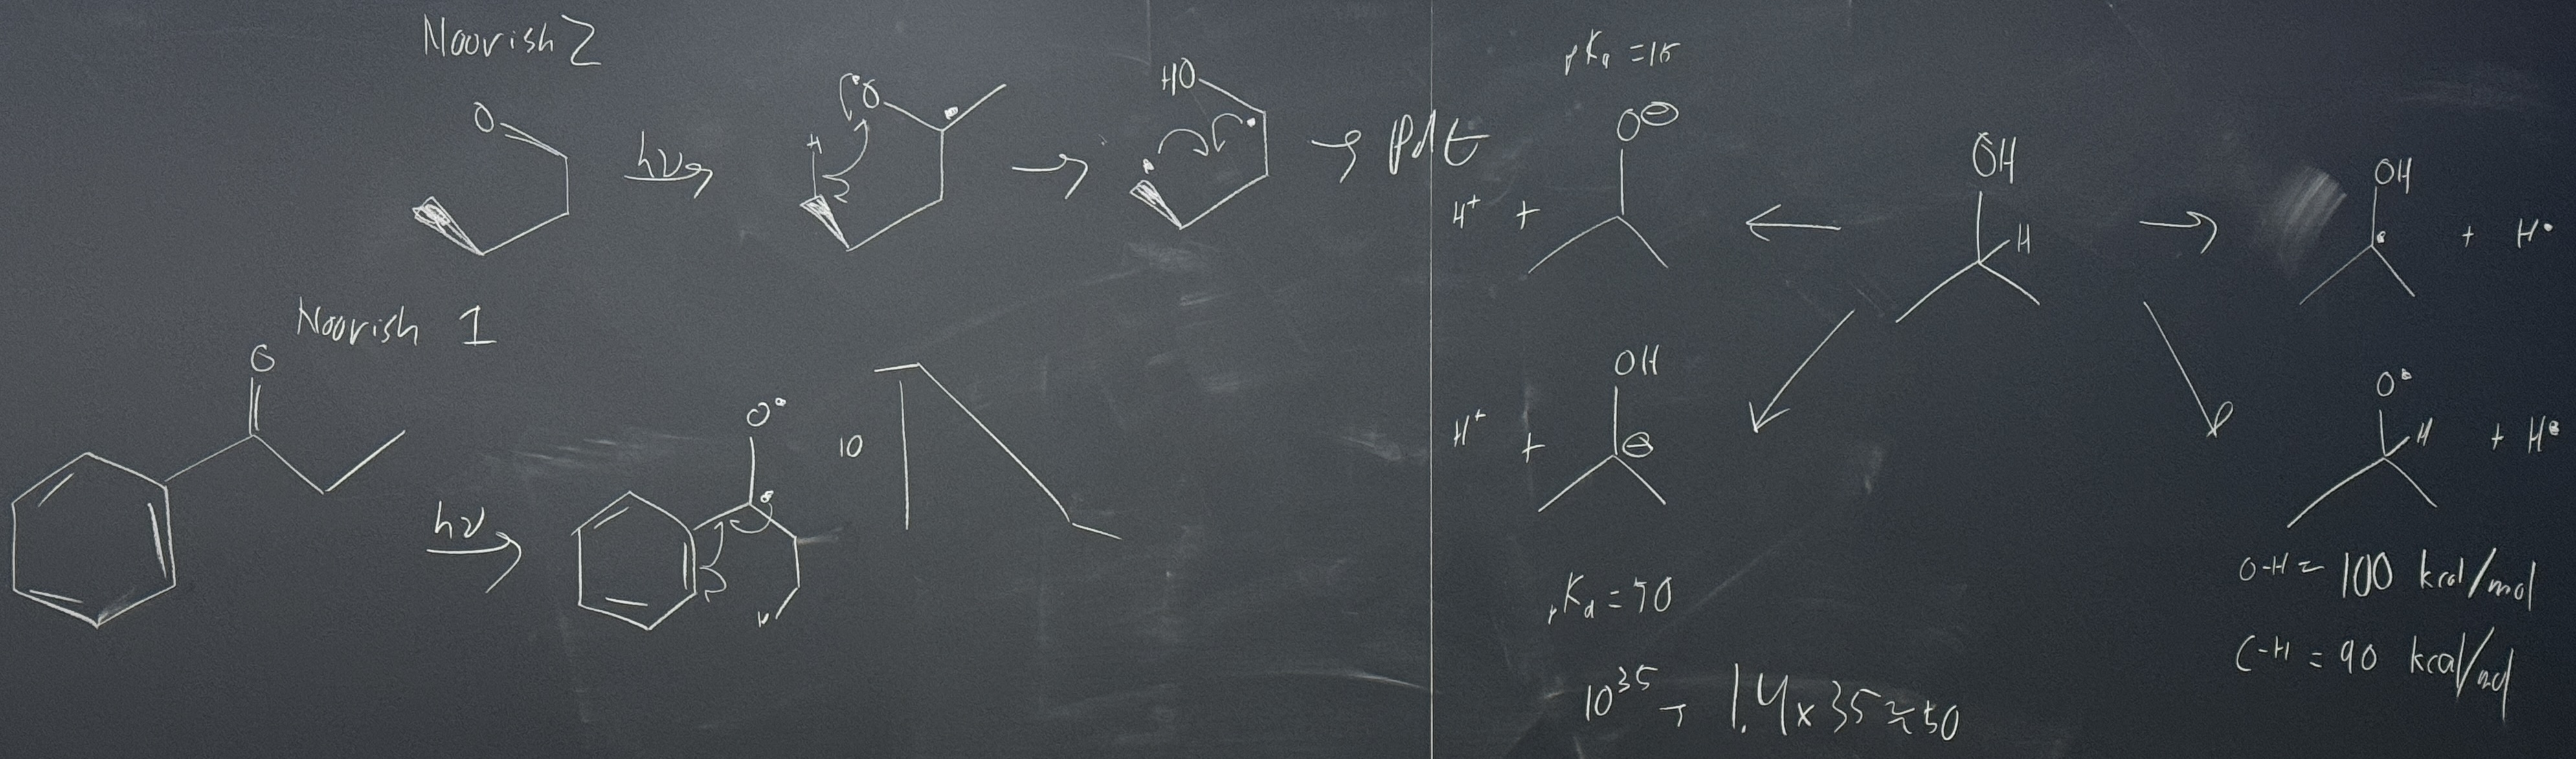
\includegraphics[width=0.8\linewidth]{WPSet1Q5S.JPG}
        \caption{Wendlandt PSet 1, Q5 solution.}
        \label{fig:WPSet1Q5S}
    \end{figure}
    \pagebreak
    \item We now begin discussing Problem 3.
    \begin{figure}[h!]
        \centering
        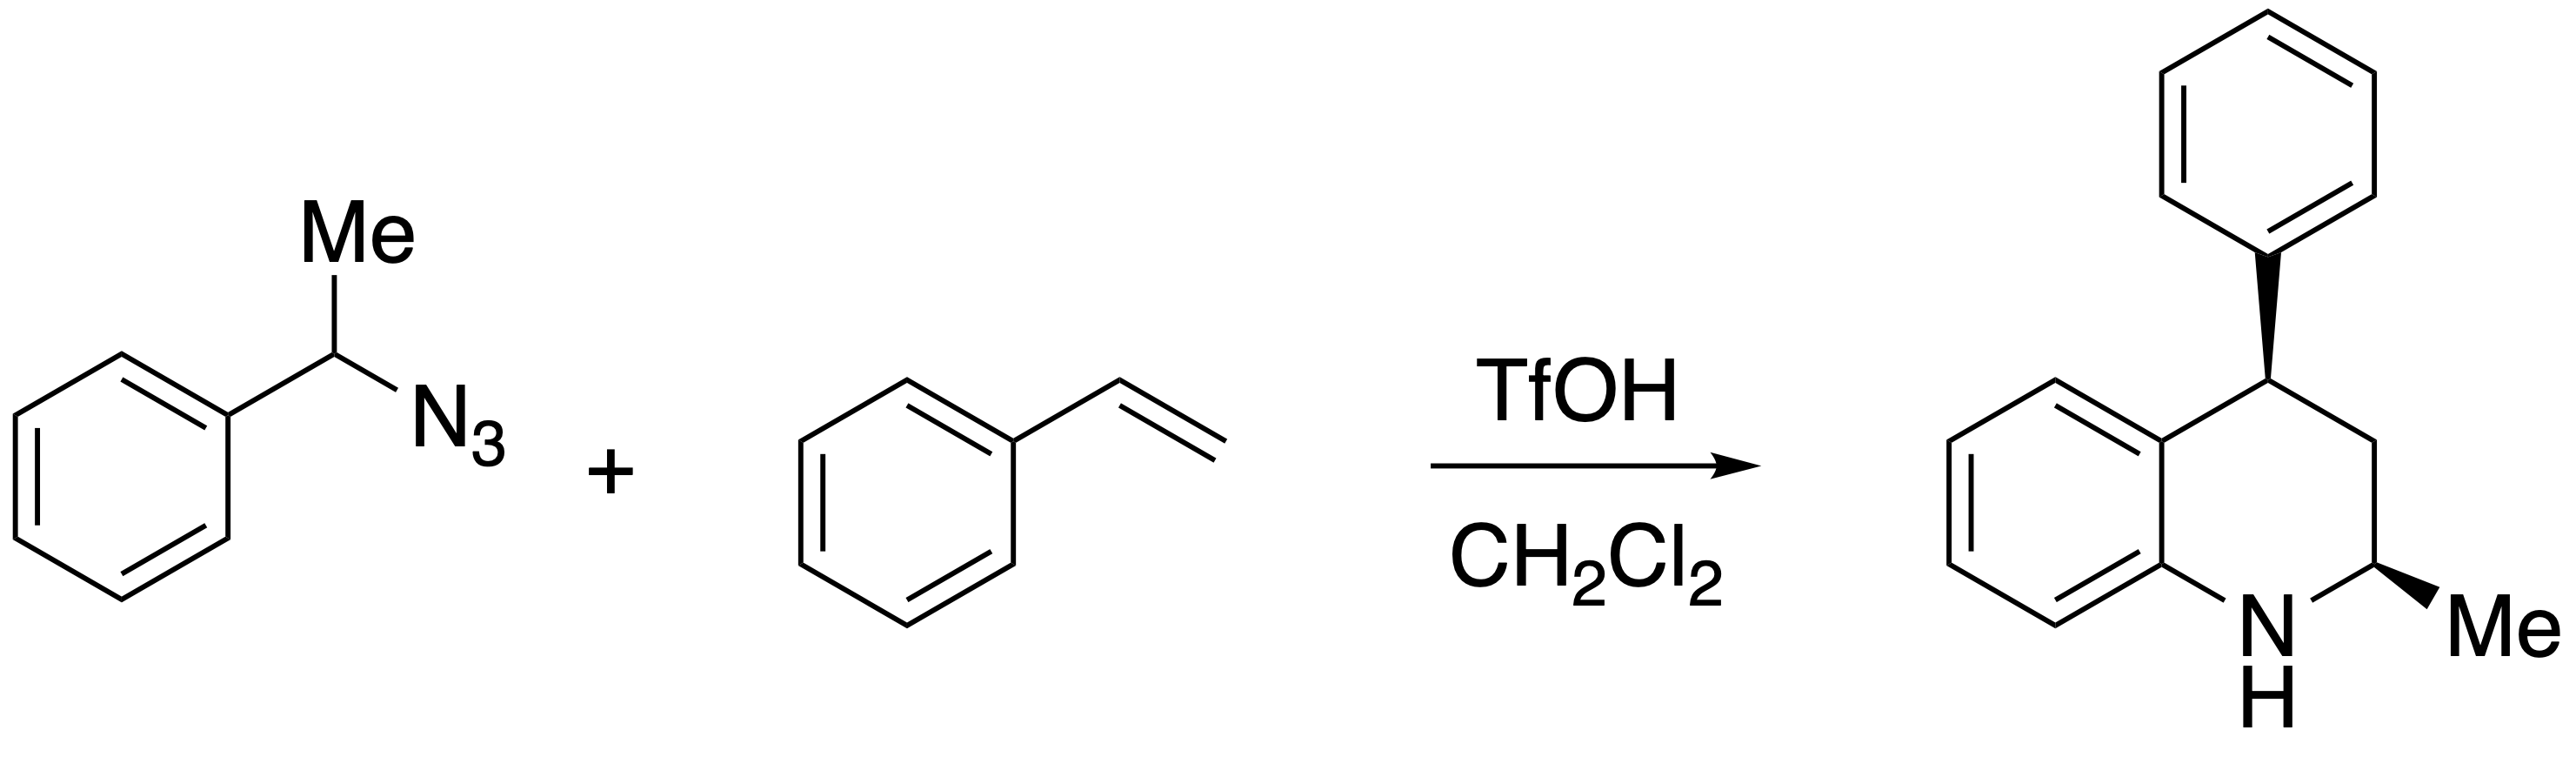
\includegraphics[width=0.55\linewidth]{WPSet1Q3.png}
        \caption{Wendlandt PSet 1, Q3.}
        \label{fig:WPSet1Q3}
    \end{figure}
    \item This reaction has a name, per Alison.
    \item When can \ce{C-C} bonds migrate?
    \item The second resonance structure explains why you protonate the internal nitrogen instead of the terminal one.
    \item The second step is $\alpha$-elimination; electrons flow from the atom to itself.
    \item Aside: Drawing an unprotonated \textbf{nitrene} (nitrogen analogue of a carbene).
    \begin{itemize}
        \item Nitrenes are electrophiles because they have one lone pair and two unpaired electrons.
        \item Nitrenes are $sp^2$-hybridized; we know this because ??.
        \begin{itemize}
            \item We'll cover this next time.
            \item 3 vs. 2 regions of electron density?
        \end{itemize}
        \item Lone pair in both $sp^2$ orbitals, vs. lone pair in one $sp$-orbital and two single electrons in orthogonal $p$ orbitals. Singlet vs. triplet nitrene.
        \item Triplet nitrene is low energy per Hund's rule; singlet nitrene is higher energy.
        \item Orbital mixing in singlet vs. triplet states. Draw an MO diagram! Next time, we'll build MOs from the ground up for nitrene.
    \end{itemize}
    \item Altogether, the full solution to PSet 1, Q3 is on the next page.
    \begin{figure}[h!]
        \centering
        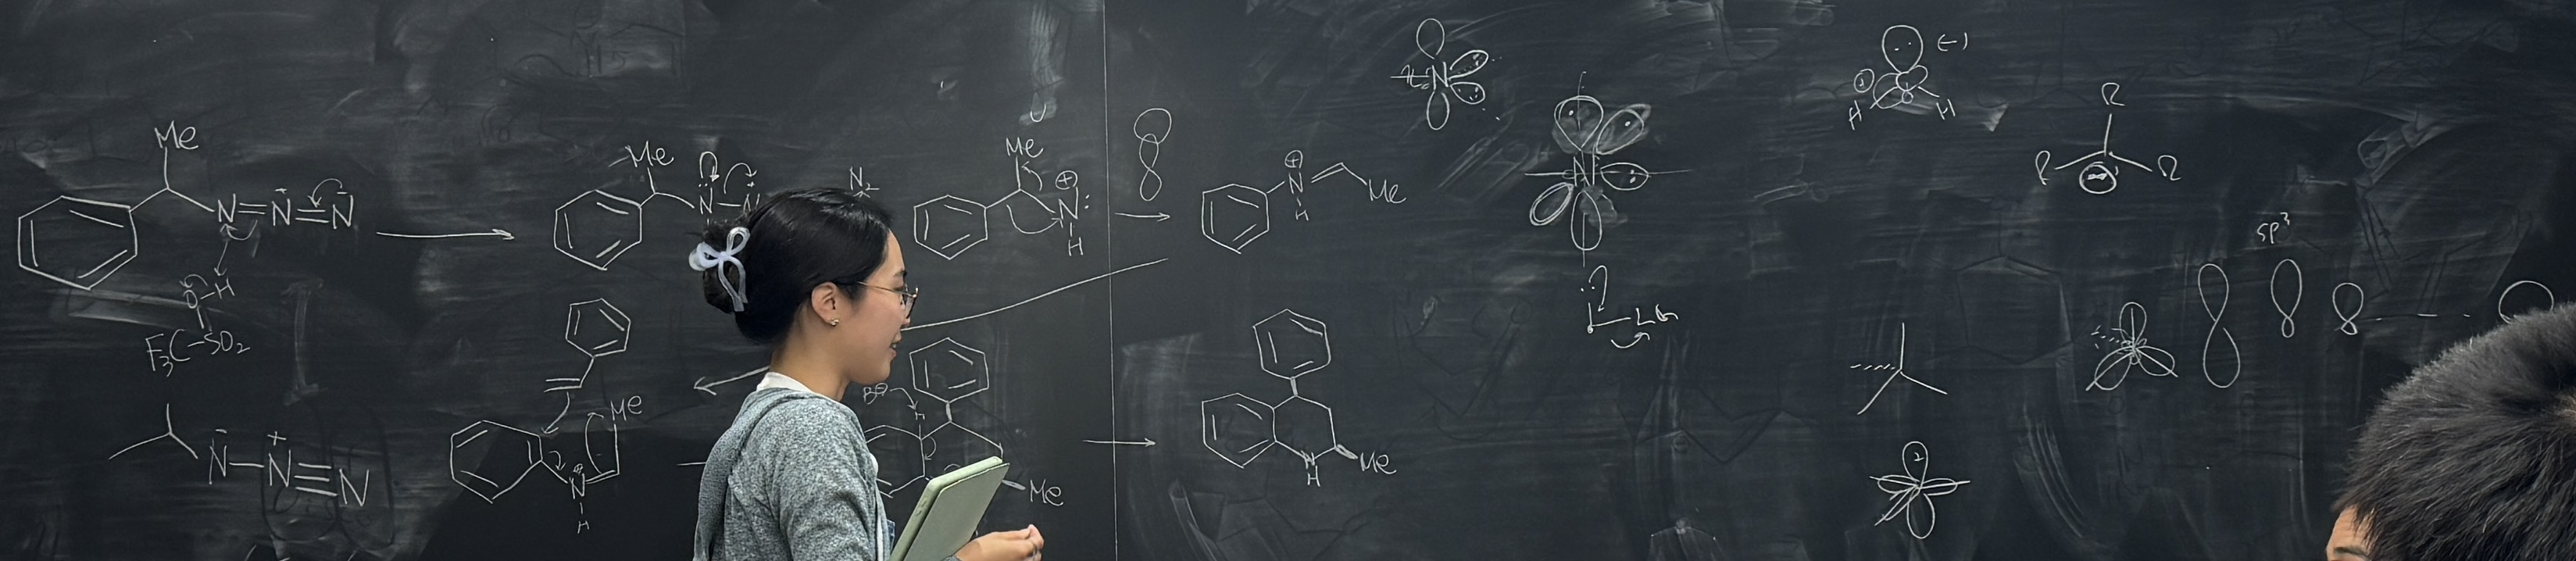
\includegraphics[width=0.8\linewidth]{WPSet1Q3S.JPG}
        \caption{Wendlandt PSet 1, Q3 solution.}
        \label{fig:WPSet1Q3S}
    \end{figure}
    \pagebreak
    \item Alison will send out PSet 2 over the weekend.
\end{itemize}



\section{Problems 9 and 10}
\begin{itemize}
    \item \marginnote{9/23:}PSet 2, Q1: Great place to use molecular model kits.
    \item We now begin discussing Problem 10.
    \begin{figure}[h!]
        \centering
        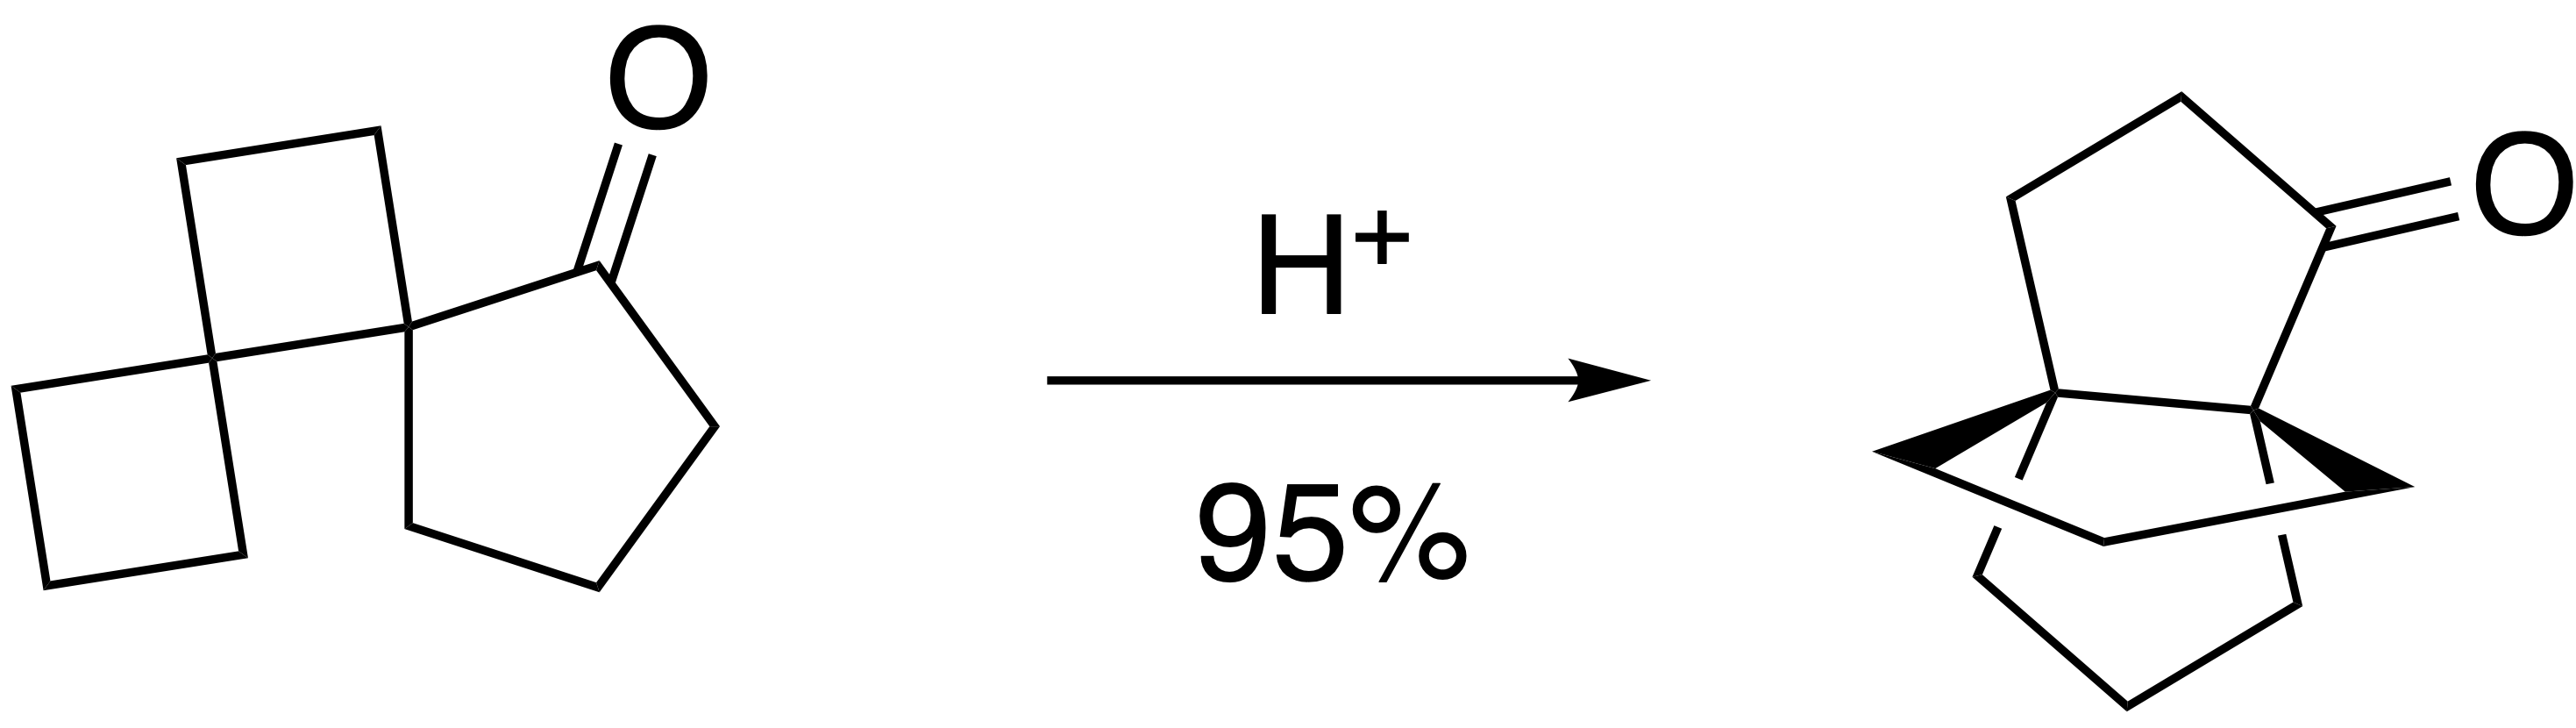
\includegraphics[width=0.35\linewidth]{WPSet1Q10.png}
        \caption{Wendlandt PSet 1, Q10.}
        \label{fig:WPSet1Q10}
    \end{figure}
    \item The final product molecule is called a \textbf{propellane} (or something like that; like a propeller).
    \item The first step is reversible.
    \begin{itemize}
        \item Alison asks about the $\pKa$ of a protonated carbonyl again.
    \end{itemize}
    \item What would be a good acid to use?
    \begin{itemize}
        \item An acid stronger than the $\pKa$ of a protonated carbonyl would be great, but we don't have many of them.
        \begin{itemize}
            \item Perhaps \ce{TsOH}??
        \end{itemize}
        \item $\pKa=-\log\Ka$.
        \begin{itemize}
            \item Recall also $\Delta G=-RT\ln\Keq\approx-1.4\log\Keq$.
        \end{itemize}
        \item Note that for a kinetically efficient process, we might not need much acid at all!
    \end{itemize}
    \item Alison has Christina draw an energy diagram again.
    \item An analysis of which steps are reversible: The ones with small differences in ring strain.
    \begin{itemize}
        \item So the product-selective steps are a bit tricky to figure out.
    \end{itemize}
    \item The resonance-stabilized carbocation is ?? times more stable than the tertiary carbocation, which is inductively stabilized via hyperconjugation.
    \begin{itemize}
        \item Alison has Christina draw an MO picture of hyperconjugation.
        \item \textbf{Mayr electrophilicity scale}.
    \end{itemize}
    \item Procedure for this problem.
    \begin{itemize}
        \item Get all the connections right.
        \item Think about the energy surface we're operating on (thermoneutral, downhill, uphill).
        \item This should give us reversibility/irreversibility.
    \end{itemize}
    \item Steven: It's easier to migrate a bond through-bond than through space.
    \begin{itemize}
        \item We never have a pure, unfilled $p$-orbital.
        \item Rather, we always have the "partial double bond" that is hyperconjugation.
        \item The carbocation changes the behavior of the entire molecule, leaning bonds in.
        \item This becomes a transition state structure for the hydride shift!
        \item TS is a 3c-2e transition state structure. This is a \textbf{nonclassical} carbocation that's much more realistic; we'll see this in 5.53. Indeed, we should \emph{not} think of carbocations as localized but very much as delocalized regions of positive charge in the local chemical environment.
        \item "In the right molecule, anything can happen." But through-space stabilization of a carbocation is much harder.
    \end{itemize}
    \item Steven: Is there a such thing as a hydroxide shift?
    \begin{itemize}
        \item We can't really do that in one step\dots but we can do it through an epoxide formation and subsequent ring opening!
    \end{itemize}
    \item David: Is there a preference for a hydride shift or a methyl shift?
    \begin{itemize}
        \item In both cases, we'll make the same tertiary carbocation.
        \item We need to think about both sterics and electronics.
        \item Electronically, \ce{C-C} bonds are more electron-rich.
        \begin{itemize}
            \item But a methyl group is also bulkier.
        \end{itemize}
        \item Thus, all else being equal (as in the example), both shifts are reasonable.
    \end{itemize}
    \item This reaction is 95\% yield due to the thermodynamic driving force, but a lot of energy went into making the initial high-energy structure.
    \item Terpene cyclizations are very hard to do without enzymes, because we have a big endergonic step to start and then lots of little downhill steps.
    \item Frank: With respect to the acid, ...
    \begin{itemize}
        \item Cross-coupling pre-Buchwald ligands buys you out of a low-energy, pre-equilibrium state.
    \end{itemize}
    \item Altogether, the full solution to PSet 1, Q10 is on the next page.
    \begin{figure}[H]
        \centering
        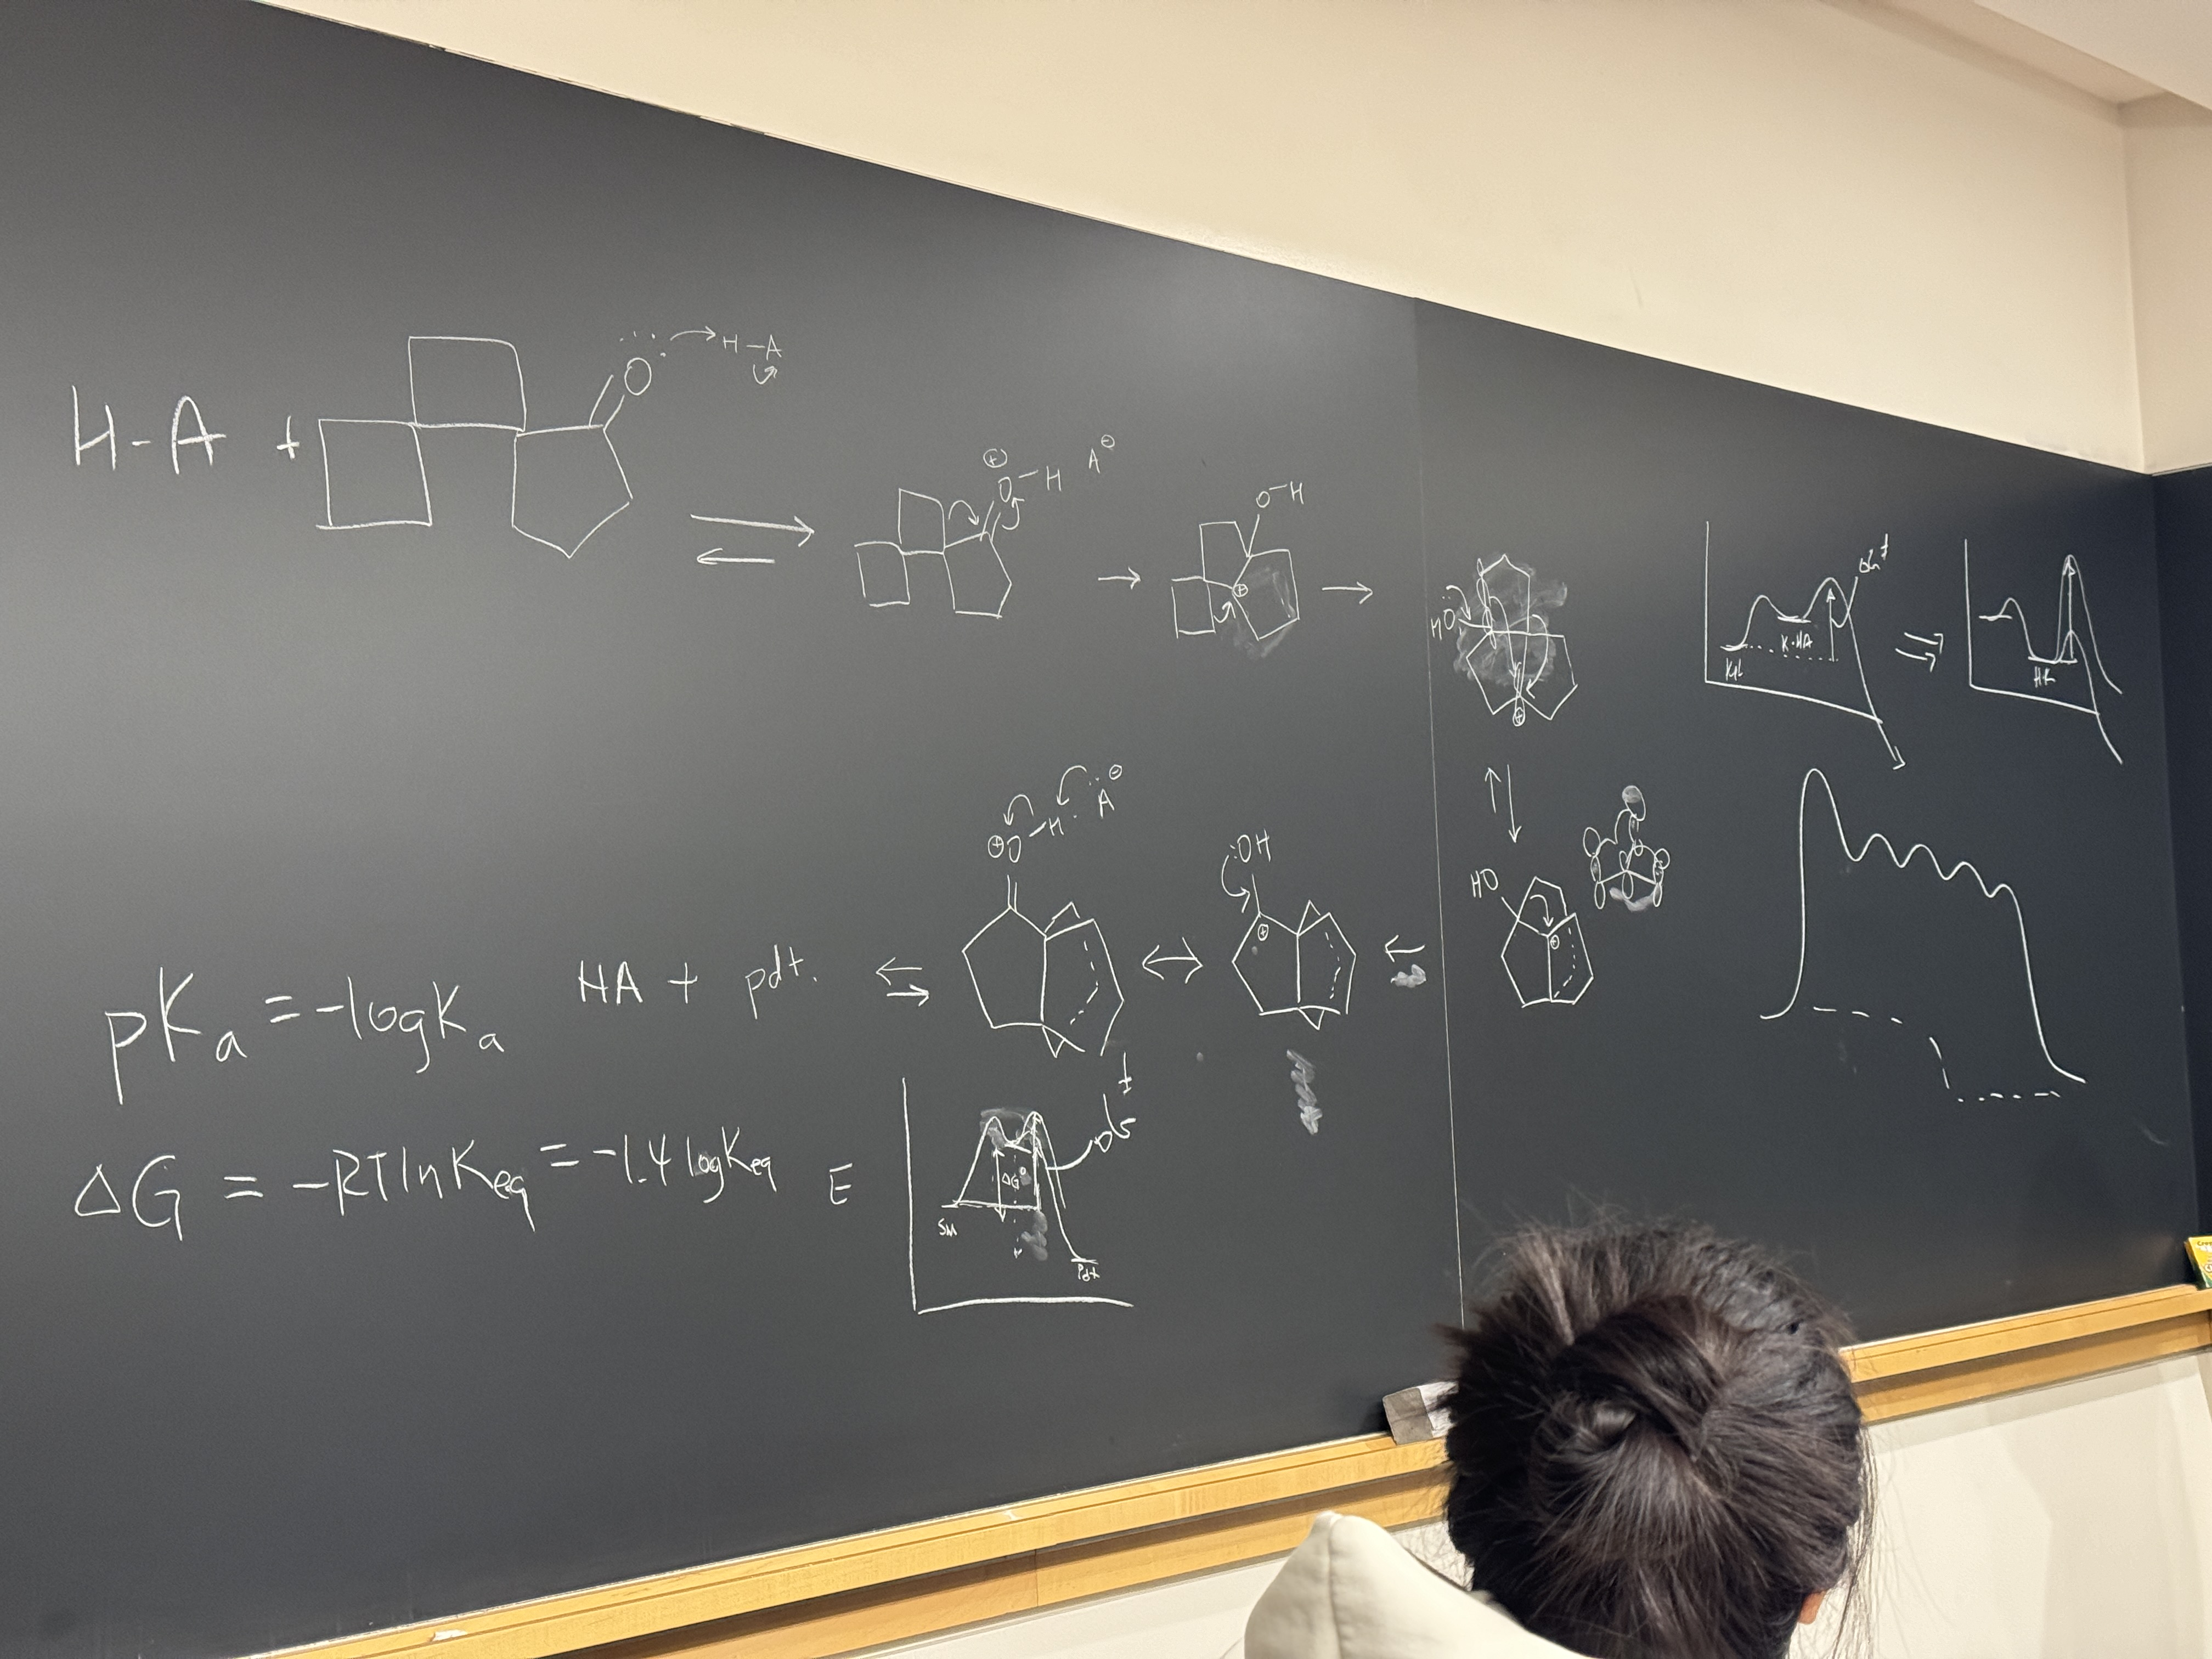
\includegraphics[width=0.8\linewidth]{WPSet1Q10S.JPG}
        \caption{Wendlandt PSet 1, Q10 solution.}
        \label{fig:WPSet1Q10S}
    \end{figure}
    \pagebreak
    \item We now begin discussing Problem 9.
    \begin{figure}[h!]
        \centering
        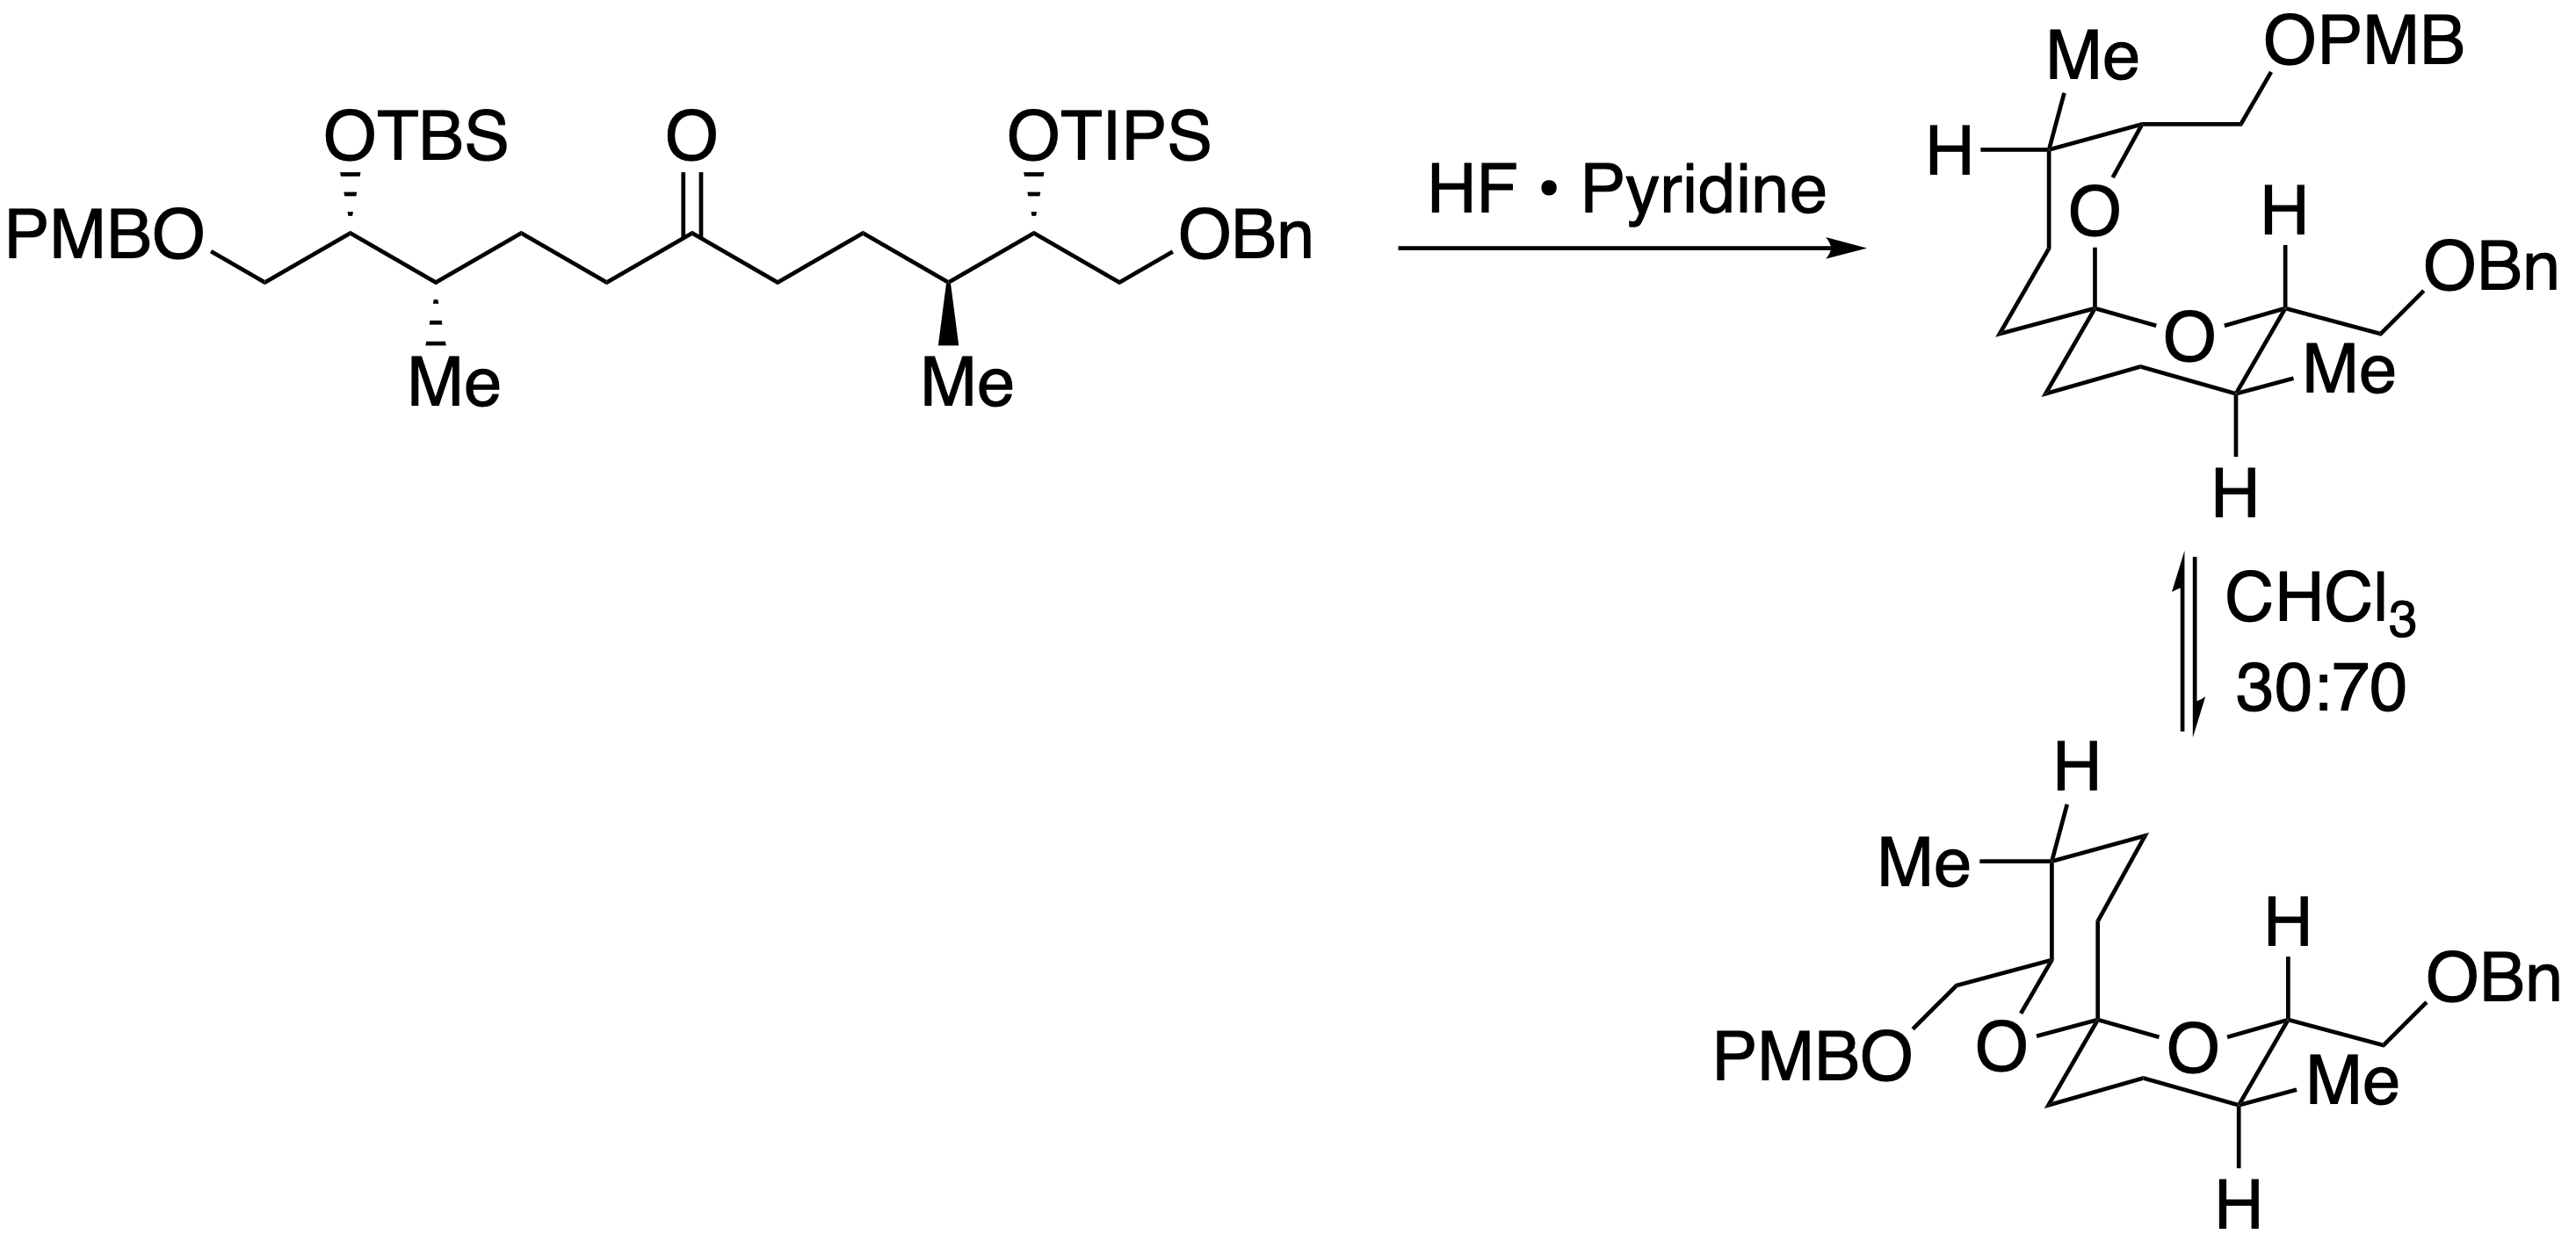
\includegraphics[width=0.65\linewidth]{WPSet1Q9.png}
        \caption{Wendlandt PSet 1, Q9.}
        \label{fig:WPSet1Q9}
    \end{figure}
    \item First step is deprotection: We lose TBS before we'll lose TIPS. Here's why.
    \item Consider some common protecting groups: \textbf{TMS}, \textbf{TES}, \textbf{TBS}, \textbf{TIPS}, and \textbf{TBDPS}.
    \begin{figure}[h!]
        \centering
        \footnotesize
        \begin{subfigure}[b]{0.17\linewidth}
            \centering
            \chemfig{Si(-[:150])(<[2])(<:[:30])-[6]!{wave}}
            \caption{TMS.}
            \label{fig:silylPGa}
        \end{subfigure}
        \begin{subfigure}[b]{0.17\linewidth}
            \centering
            \chemfig{Si(-[:150]-[::60])(<[2]-[::60])(<:[:30]-[::-60])-[6]!{wave}}
            \caption{TES.}
            \label{fig:silylPGb}
        \end{subfigure}
        \begin{subfigure}[b]{0.17\linewidth}
            \centering
            \chemfig{Si(-[:150])(<[2](-[::60])(<[::0])(<:[::-60]))(<:[:30])-[6]!{wave}}
            \caption{TBS.}
            \label{fig:silylPGc}
        \end{subfigure}
        \begin{subfigure}[b]{0.17\linewidth}
            \centering
            \chemfig{Si(-[:150](-[::60])(-[::-60]))(<[2](-[::60])(-[::-60]))(<:[:30](-[::60])(-[::-60]))-[6]!{wave}}
            \caption{TIPS.}
            \label{fig:silylPGd}
        \end{subfigure}
        \begin{subfigure}[b]{0.17\linewidth}
            \centering
            \chemfig{Si(-[:150]Ph)(<[2](-[::60])(<[::0])(<:[::-60]))(<:[:30]Ph)-[6]!{wave}}
            \caption{TBDPS.}
            \label{fig:silylPGe}
        \end{subfigure}
        \caption{Silyl protecting groups.}
        \label{fig:silylPG}
    \end{figure}
    \item \textbf{Trimethylsilane}. \emph{Denoted by} \textbf{TMS}. \emph{Given by} Figure \ref{fig:silylPGa}.
    \item \textbf{Triethylsilane}. \emph{Denoted by} \textbf{TES}. \emph{Given by} Figure \ref{fig:silylPGb}.
    \item \textbf{\textsuperscript{\emph{t}}Butyldimethylsilane}. \emph{Denoted by} \textbf{TBS}. \emph{Given by} Figure \ref{fig:silylPGc}.
    \item \textbf{Triisopropylsilane}. \emph{Denoted by} \textbf{TIPS}. \emph{Given by} Figure \ref{fig:silylPGd}.
    \item \textbf{\textsuperscript{\emph{t}}Butyldiphenylsilane}. \emph{Denoted by} \textbf{TBDPS}. \emph{Given by} Figure \ref{fig:silylPGe}.
    \item Relative stability against hydrolysis in acidic media.
    \begin{itemize}
        \item $\text{TMS}:\text{TES}:\text{TBS}:\text{TIPS}:\text{TBDPS}$ is $1:64:\num{2000}:\num{700000}:\num{5000000}$.
    \end{itemize}
    \item TBDPS was developed for carbohydrate chemistry, because they needed something that wouldn't fall off!
    \item We get to the product as expected.
    \item Now let's rationalize the ratio.
    \begin{itemize}
        \item The second product is doubly anomeric.
        \item Substituents want to be equatorial, as well.
        \item With axial OPMB, two H's point right at each other. And they are locked into space this way due to the \emph{spiro}-ketal.
        \item We also have to consider solvent effects.
        \begin{itemize}
            \item \ce{CHCl3} has a relatively high \textbf{dielectric} ($\sim 4$), and hence is relatively nonpolar.
            \item Look up the \textbf{dielectric effect} in chemistry!!
        \end{itemize}
        \item Solvent dipole and molecular dipole matters in PSet 2, Q1, too!
    \end{itemize}
    \item Indeed, chloroform is a polar molecule but a nonpolar \emph{solvent} because it is not miscible with water and has a low dielectric constant. However, it is polar compared to many other organic solvents!
    \item Sterics only becomes a problem when things are "literally right on top of each other."
    \emph{picture; \ce{H2} PE surface}.
    \begin{itemize}
        \item Bond angles matter more in most molecules!
        \item You get a lot more out of bringing things close together until you \emph{really} pay.
        \item Takeaway: Bringing two things together is very often stabilizing (dipolar/quadripolar interactions, LDFs, etc.). We generally get this wrong.
    \end{itemize}
    \item Altogether, the full solution to PSet 1, Q9 is on the next page.
    \begin{figure}[h!]
        \centering
        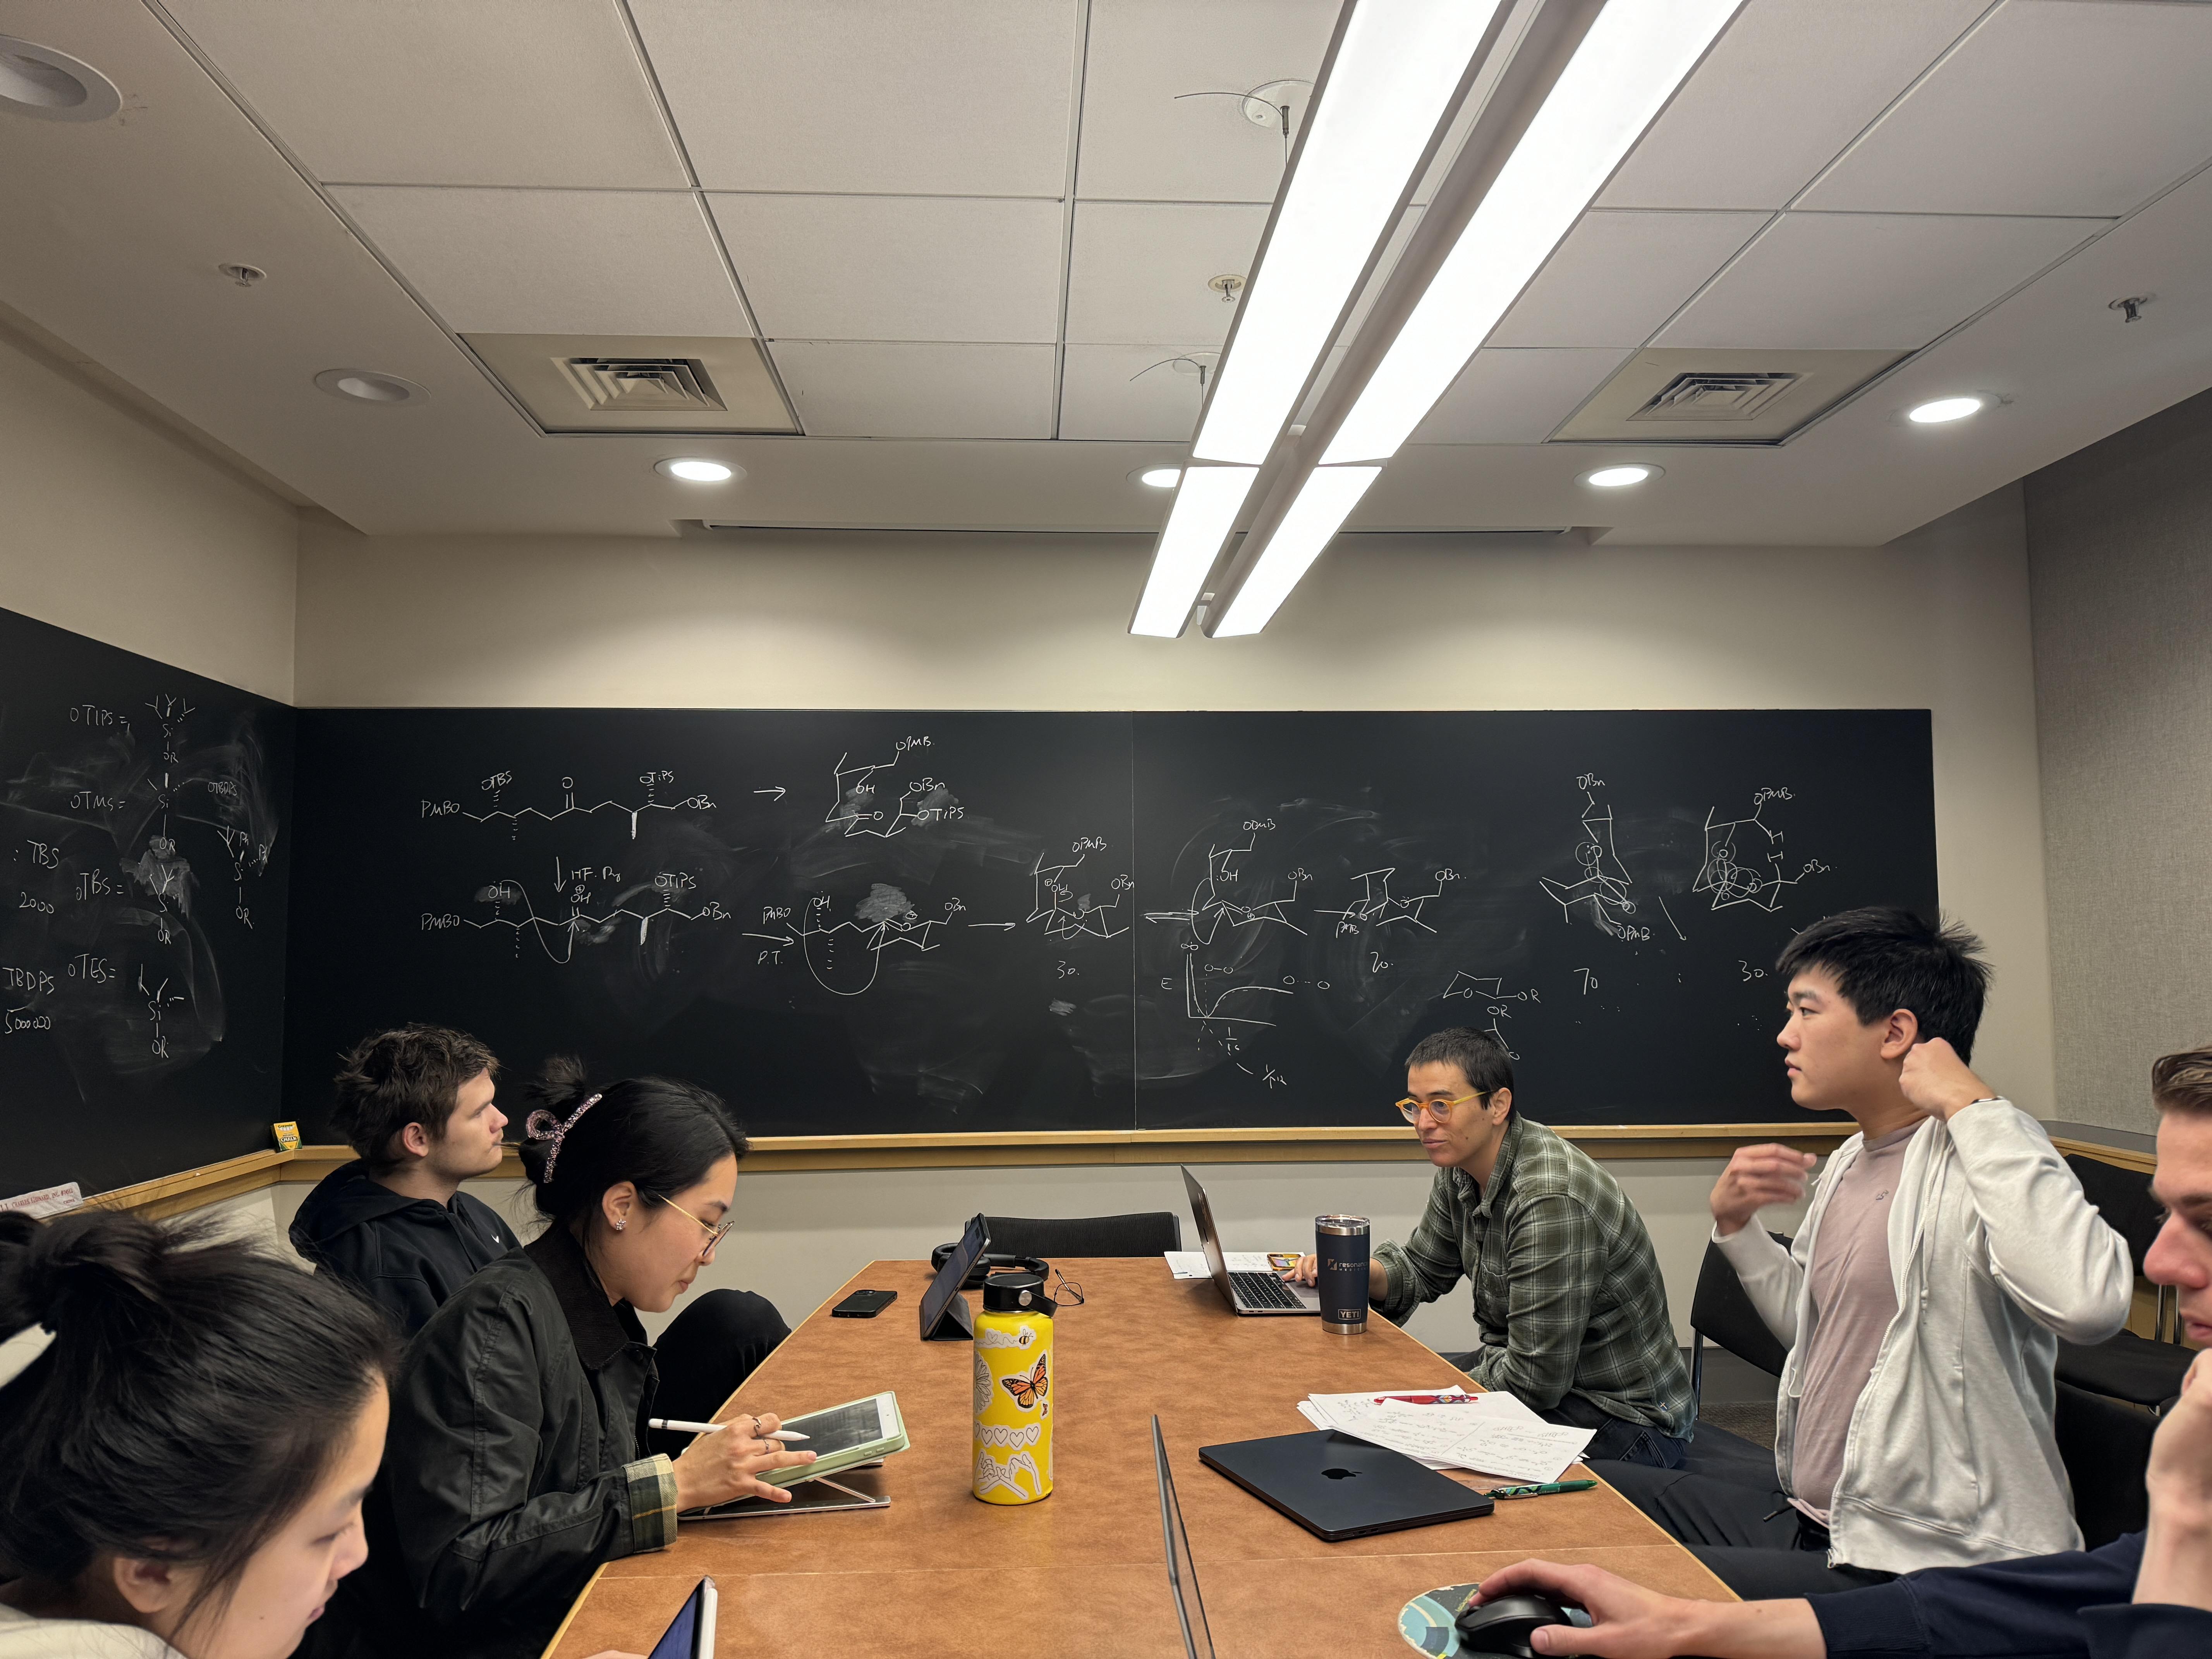
\includegraphics[width=0.8\linewidth]{WPSet1Q9S.JPG}
        \caption{Wendlandt PSet 1, Q9 solution.}
        \label{fig:WPSet1Q9S}
    \end{figure}
    \pagebreak
    \item We now pick up last time's discussion on nitrenes, from Problem 3 (Figure \ref{fig:WPSet1Q3}).
    \item \textbf{Povarov reaction}.
    \item Think about arrow pushing in terms of which electrons are moving from which orbital to which other orbital.
    \begin{itemize}
        \item In the rearrangement step, electrons leave from the \ce{Ar-C} bond and go into the nitrogen's empty, positively charged $p$-orbital.
        \begin{itemize}
            \item They don't go into the \ce{N-H} $\sigma^*$ orbital because that kind of S\textsubscript{N}2 attack would kick out \ce{H-}.
            \item There's also another option we can rule out.
        \end{itemize}
        \item Then electrons leave from the nitrogen lone pair and move into a new $\pi$-bond.
    \end{itemize}
    \item Why does the aryl group migrate instead of the methyl group?
    \begin{itemize}
        \item Because it forms a resonance-stabilied carbocation??
        \item Specifically, we get a \textbf{phenonium ion} that stabilizes the positive charge through delocalization.
    \end{itemize}
    \item Alison "numbers the shit" out of structures she's working on; there's no shame in it.
    \item Jasmin \emph{really} can't think on her feet.
    \item $[4+2]$ cycloaddition in the end.
    \item Aside: Suffixes.
    \begin{itemize}
        \item Three examples.
        \begin{itemize}
            \item -ium: Cation.
            \item -yl: Radical.
            \item -ide: Anion.
        \end{itemize}
        \item So "phenyl" technically means the phenyl radial.
        \item This also explains the difference between "hydroxyl" and "hydroxide"
    \end{itemize}
\end{itemize}



\section{Problem 2}
\begin{itemize}
    \item \marginnote{9/25:}Starting with Jasmin's azide one again.
    \item Normal vs. \textbf{inverse electron-demand Diels-Alder}.
    \begin{itemize}
        \item This reaction is an inverse electron-demand Diels-Alder because the HOMO of the diene is so stabilized that the electrons from the dienophile HOMO will donate into the LUMO of the diene.
        \item The diene HOMO is dropped so much because of the electron withdrawing nitrogen in the conjugated system.
        \item The dienophile is electron rich because it's styrene, and that's pretty electron rich.
    \end{itemize}
    \item A concerted Diels-Alder would break aromaticity, and you'd have steric clash to the desired product, so perhaps that's disfavored. Though, I think Alison's DA stereochemistry might be backwards...
    \item \textbf{Twist-boat} (transition state diagram): ??
    \item DA regiochemistry is defined by the \textbf{orbital coefficient}, i.e., the $\delta^+$ and $\delta^-$.
    \item To a first approximation, a reasonably stable cation followed by a Friedel-Crafts type end to aromaticity is probably more defensible than a DA that breaks aromaticity.
    \item We now begin discussing Problem 2.
    \begin{figure}[h!]
        \centering
        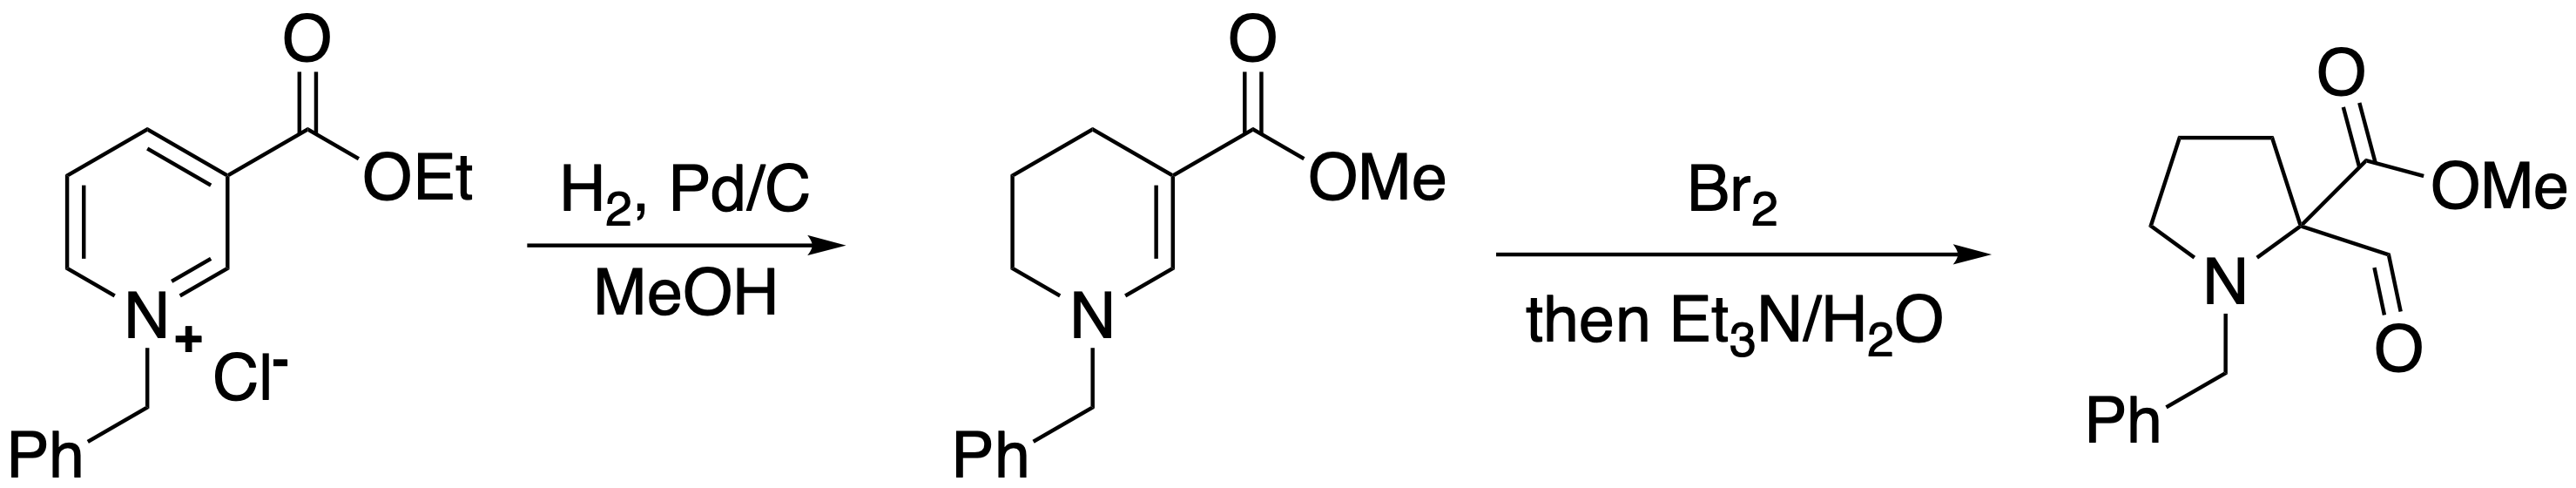
\includegraphics[width=0.75\linewidth]{WPSet1Q2.png}
        \caption{Wendlandt PSet 1, Q2.}
        \label{fig:WPSet1Q2}
    \end{figure}
    \item First step: The hydrogenation.
    \begin{itemize}
        \item It's not that you have insufficient kinetic access to reduce the product; it's that you have a very deactivated pyridinium, and the product is actually more stable since it's so highly conjugated.
        \item The pyridinium is \textbf{cross-conjugated}, as well.
        \item We'll also have transesterification.
    \end{itemize}
    \item The product is a racemate, so we can track stereochemistry through the mechanism but assign it arbitrarily. In other words, just be consistent, and then understand that the product will contain both enantiomers.
    \item Bromonium ion is broken by the lone pair from the nearby nitrogen. Then water adds in to form the hemiaminal.
    \item Hydrolysis of the hemiaminal yields the aldehyde.
    \item Then an S\textsubscript{N}2 or S\textsubscript{N}1 attack can close the 5-membered ring.
    \begin{itemize}
        \item Alternatively, consider an intramolecular, through-bond \ce{C-N} migration.
        \item Leaving groups $\alpha$ to carbonyl groups are exceptionally good electrophiles for S\textsubscript{N}2.
        \begin{itemize}
            \item We can rationalize this via orbitals.
            \item One idea: Donation from the \ce{C=O} $\pi$-orbital to the \ce{C-Br} $\sigma^*$ orbital weakens that bond.
            \item Another idea: Consider the transition state. The \textbf{A value} of methyl, ethyl, and isopropyl are all quite similar. Bromine is much smaller (0.83) vs. ester (1.73), so this 1 kcal difference in free energy gives us a $10:1$ preference for equatorial ester. The reaction can only go with equatorial bromine, though.
            \item \textbf{Curtin-Hammett kinetic scenario}.
        \end{itemize}
    \end{itemize}
    \item \textbf{A value}: An empirical measure of how much a substituent on a cyclohexane likes to be axial or equatorial.
    \begin{itemize}
        \item Essentially, this is a net measure of a whole bunch of different effects that cause the free energy difference between the two ring conformers.
    \end{itemize}
    \item Altogether, the full solution to PSet 1, Q2 is on the next page.
    \begin{figure}[H]
        \centering
        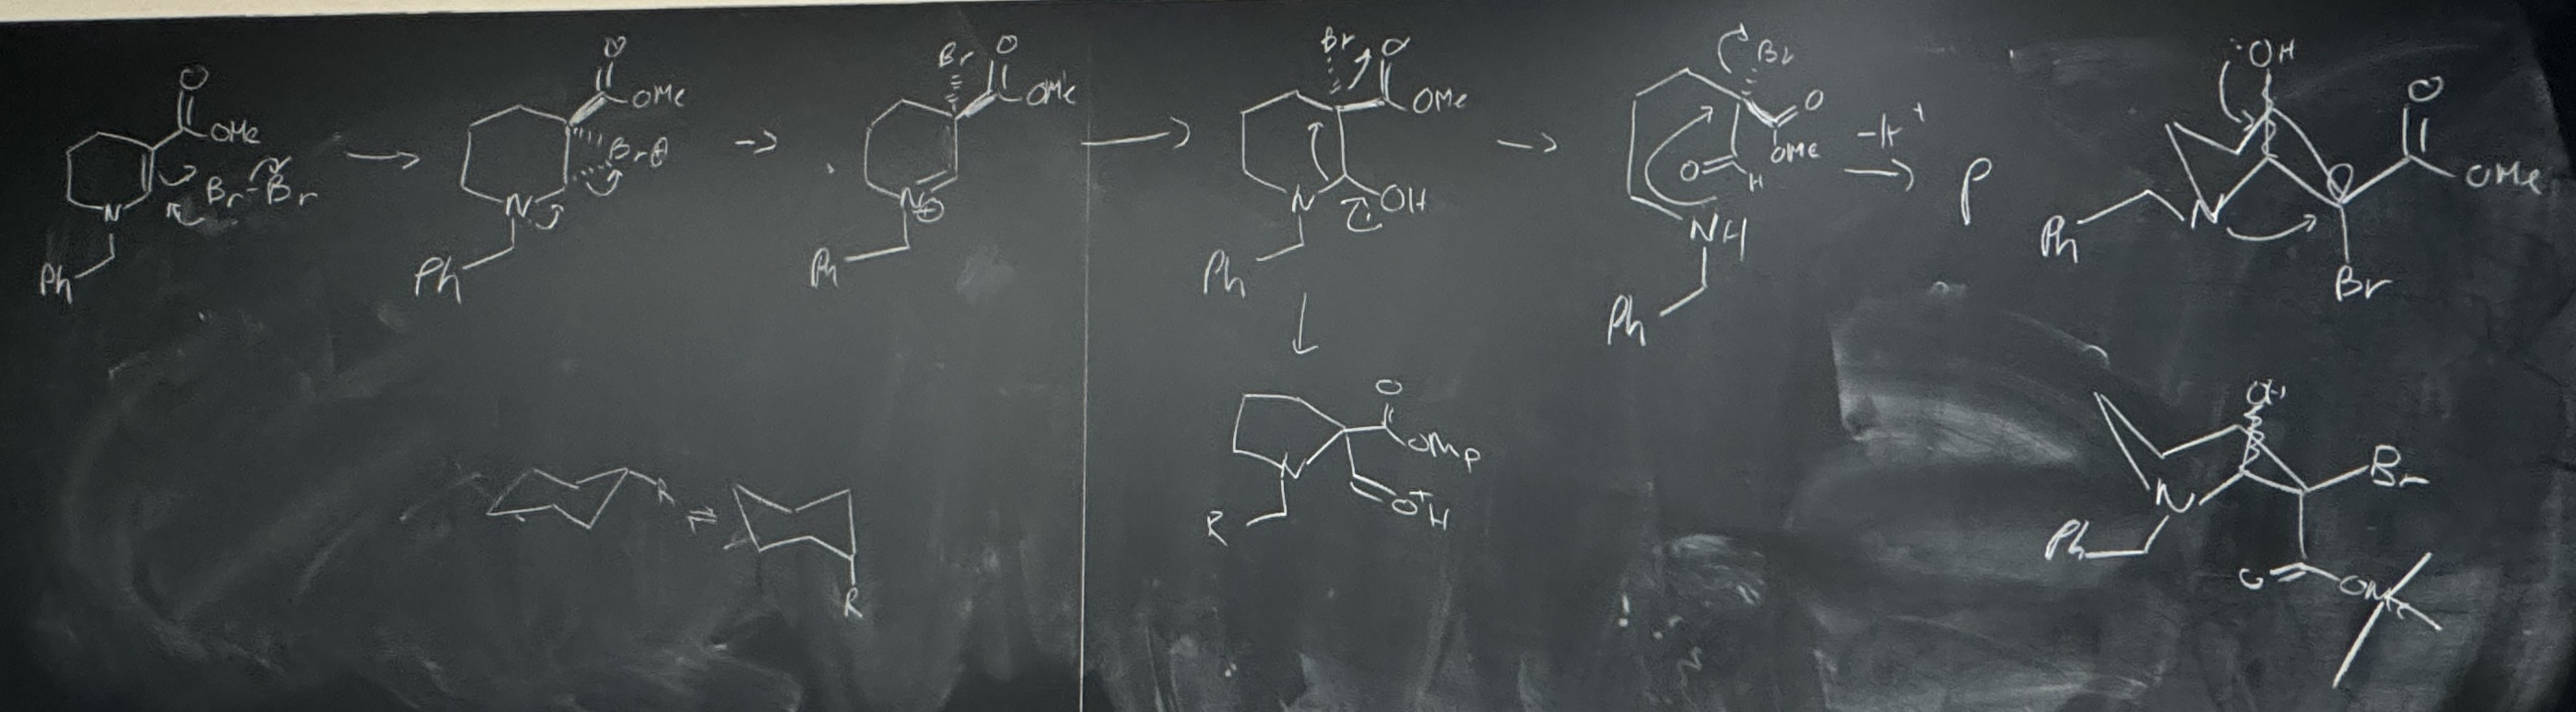
\includegraphics[width=0.8\linewidth]{WPSet1Q2S.JPG}
        \caption{Wendlandt PSet 1, Q2 solution.}
        \label{fig:WPSet1Q2S}
    \end{figure}
    \pagebreak
    \item Alison's PSets are way more open-ended than Mo's because she doesn't like arrow-pushing mechanisms.
\end{itemize}




\end{document}